% Options for packages loaded elsewhere
\PassOptionsToPackage{unicode}{hyperref}
\PassOptionsToPackage{hyphens}{url}
\PassOptionsToPackage{dvipsnames,svgnames,x11names}{xcolor}
%
\documentclass[
]{agujournal2019}

\usepackage{amsmath,amssymb}
\usepackage{iftex}
\ifPDFTeX
  \usepackage[T1]{fontenc}
  \usepackage[utf8]{inputenc}
  \usepackage{textcomp} % provide euro and other symbols
\else % if luatex or xetex
  \usepackage{unicode-math}
  \defaultfontfeatures{Scale=MatchLowercase}
  \defaultfontfeatures[\rmfamily]{Ligatures=TeX,Scale=1}
\fi
\usepackage{lmodern}
\ifPDFTeX\else  
    % xetex/luatex font selection
\fi
% Use upquote if available, for straight quotes in verbatim environments
\IfFileExists{upquote.sty}{\usepackage{upquote}}{}
\IfFileExists{microtype.sty}{% use microtype if available
  \usepackage[]{microtype}
  \UseMicrotypeSet[protrusion]{basicmath} % disable protrusion for tt fonts
}{}
\makeatletter
\@ifundefined{KOMAClassName}{% if non-KOMA class
  \IfFileExists{parskip.sty}{%
    \usepackage{parskip}
  }{% else
    \setlength{\parindent}{0pt}
    \setlength{\parskip}{6pt plus 2pt minus 1pt}}
}{% if KOMA class
  \KOMAoptions{parskip=half}}
\makeatother
\usepackage{xcolor}
\setlength{\emergencystretch}{3em} % prevent overfull lines
\setcounter{secnumdepth}{5}
% Make \paragraph and \subparagraph free-standing
\makeatletter
\ifx\paragraph\undefined\else
  \let\oldparagraph\paragraph
  \renewcommand{\paragraph}{
    \@ifstar
      \xxxParagraphStar
      \xxxParagraphNoStar
  }
  \newcommand{\xxxParagraphStar}[1]{\oldparagraph*{#1}\mbox{}}
  \newcommand{\xxxParagraphNoStar}[1]{\oldparagraph{#1}\mbox{}}
\fi
\ifx\subparagraph\undefined\else
  \let\oldsubparagraph\subparagraph
  \renewcommand{\subparagraph}{
    \@ifstar
      \xxxSubParagraphStar
      \xxxSubParagraphNoStar
  }
  \newcommand{\xxxSubParagraphStar}[1]{\oldsubparagraph*{#1}\mbox{}}
  \newcommand{\xxxSubParagraphNoStar}[1]{\oldsubparagraph{#1}\mbox{}}
\fi
\makeatother


\providecommand{\tightlist}{%
  \setlength{\itemsep}{0pt}\setlength{\parskip}{0pt}}\usepackage{longtable,booktabs,array}
\usepackage{calc} % for calculating minipage widths
% Correct order of tables after \paragraph or \subparagraph
\usepackage{etoolbox}
\makeatletter
\patchcmd\longtable{\par}{\if@noskipsec\mbox{}\fi\par}{}{}
\makeatother
% Allow footnotes in longtable head/foot
\IfFileExists{footnotehyper.sty}{\usepackage{footnotehyper}}{\usepackage{footnote}}
\makesavenoteenv{longtable}
\usepackage{graphicx}
\makeatletter
\newsavebox\pandoc@box
\newcommand*\pandocbounded[1]{% scales image to fit in text height/width
  \sbox\pandoc@box{#1}%
  \Gscale@div\@tempa{\textheight}{\dimexpr\ht\pandoc@box+\dp\pandoc@box\relax}%
  \Gscale@div\@tempb{\linewidth}{\wd\pandoc@box}%
  \ifdim\@tempb\p@<\@tempa\p@\let\@tempa\@tempb\fi% select the smaller of both
  \ifdim\@tempa\p@<\p@\scalebox{\@tempa}{\usebox\pandoc@box}%
  \else\usebox{\pandoc@box}%
  \fi%
}
% Set default figure placement to htbp
\def\fps@figure{htbp}
\makeatother
% definitions for citeproc citations
\NewDocumentCommand\citeproctext{}{}
\NewDocumentCommand\citeproc{mm}{%
  \begingroup\def\citeproctext{#2}\cite{#1}\endgroup}
\makeatletter
 % allow citations to break across lines
 \let\@cite@ofmt\@firstofone
 % avoid brackets around text for \cite:
 \def\@biblabel#1{}
 \def\@cite#1#2{{#1\if@tempswa , #2\fi}}
\makeatother
\newlength{\cslhangindent}
\setlength{\cslhangindent}{1.5em}
\newlength{\csllabelwidth}
\setlength{\csllabelwidth}{3em}
\newenvironment{CSLReferences}[2] % #1 hanging-indent, #2 entry-spacing
 {\begin{list}{}{%
  \setlength{\itemindent}{0pt}
  \setlength{\leftmargin}{0pt}
  \setlength{\parsep}{0pt}
  % turn on hanging indent if param 1 is 1
  \ifodd #1
   \setlength{\leftmargin}{\cslhangindent}
   \setlength{\itemindent}{-1\cslhangindent}
  \fi
  % set entry spacing
  \setlength{\itemsep}{#2\baselineskip}}}
 {\end{list}}
\usepackage{calc}
\newcommand{\CSLBlock}[1]{\hfill\break\parbox[t]{\linewidth}{\strut\ignorespaces#1\strut}}
\newcommand{\CSLLeftMargin}[1]{\parbox[t]{\csllabelwidth}{\strut#1\strut}}
\newcommand{\CSLRightInline}[1]{\parbox[t]{\linewidth - \csllabelwidth}{\strut#1\strut}}
\newcommand{\CSLIndent}[1]{\hspace{\cslhangindent}#1}

\usepackage{url} %this package should fix any errors with URLs in refs.
\usepackage{lineno}
\usepackage[inline]{trackchanges} %for better track changes. finalnew option will compile document with changes incorporated.
\usepackage{soul}
\linenumbers
\makeatletter
\@ifpackageloaded{float}{}{\usepackage{float}}
\floatstyle{plain}
\@ifundefined{c@chapter}{\newfloat{suppfig}{h}{losuppfig}}{\newfloat{suppfig}{h}{losuppfig}[chapter]}
\floatname{suppfig}{Figure S}
\newcommand*\quartosuppfigref[1]{Figure \hyperref[#1]{S\ref{#1}}}
\@ifpackageloaded{caption}{}{\usepackage{caption}}
\DeclareCaptionLabelFormat{quartosuppfigreflabelformat}{#1#2}
\captionsetup[suppfig]{labelformat=quartosuppfigreflabelformat}
\newcommand*\listofsuppfigs{\listof{suppfig}{List of Supplementary Figures}}
\makeatother
\makeatletter
\@ifpackageloaded{caption}{}{\usepackage{caption}}
\AtBeginDocument{%
\ifdefined\contentsname
  \renewcommand*\contentsname{Table of contents}
\else
  \newcommand\contentsname{Table of contents}
\fi
\ifdefined\listfigurename
  \renewcommand*\listfigurename{List of Figures}
\else
  \newcommand\listfigurename{List of Figures}
\fi
\ifdefined\listtablename
  \renewcommand*\listtablename{List of Tables}
\else
  \newcommand\listtablename{List of Tables}
\fi
\ifdefined\figurename
  \renewcommand*\figurename{Figure}
\else
  \newcommand\figurename{Figure}
\fi
\ifdefined\tablename
  \renewcommand*\tablename{Table}
\else
  \newcommand\tablename{Table}
\fi
}
\@ifpackageloaded{float}{}{\usepackage{float}}
\floatstyle{ruled}
\@ifundefined{c@chapter}{\newfloat{codelisting}{h}{lop}}{\newfloat{codelisting}{h}{lop}[chapter]}
\floatname{codelisting}{Listing}
\newcommand*\listoflistings{\listof{codelisting}{List of Listings}}
\makeatother
\makeatletter
\makeatother
\makeatletter
\@ifpackageloaded{caption}{}{\usepackage{caption}}
\@ifpackageloaded{subcaption}{}{\usepackage{subcaption}}
\makeatother

\usepackage{bookmark}

\IfFileExists{xurl.sty}{\usepackage{xurl}}{} % add URL line breaks if available
\urlstyle{same} % disable monospaced font for URLs
\hypersetup{
  pdftitle={Effects of Riparian Grazing on Distinct Water-Extractable Phosphorus Sources},
  pdfauthor={Alexander J Koiter; Tamaragh Y Malone},
  pdfkeywords={Phosphorus, Grazing, Riparian},
  colorlinks=true,
  linkcolor={blue},
  filecolor={Maroon},
  citecolor={Blue},
  urlcolor={Blue},
  pdfcreator={LaTeX via pandoc}}


\journalname{TBD}

\draftfalse

\begin{document}
\title{Effects of Riparian Grazing on Distinct Water-Extractable
Phosphorus Sources}

\authors{Alexander J Koiter\affil{1}, Tamaragh Y Malone\affil{2}}
\affiliation{1}{Brandon University, Department of Geography and
Environment, Brandon, MB, }\affiliation{2}{Brandon University,
Department of Biology, Brandon, MB, }
\correspondingauthor{Alexander J Koiter}{koitera@brandonu.ca}


\begin{abstract}
Riparian areas play an important role in maintaining water quality in
agricultural watersheds by buffering sediment, nutrients, and other
pollutants. Recent studies have shown that in some cases riparian areas
are a net source of phosphorus (P) in cold climates. This study assessed
the impact of cattle grazing or harvesting of riparian areas on the
spatial and vertical distribution of water-extractable phosphorus (WEP).
This study measured the WEP in four distinctive sources: biomass,
litter, organic layer, and Ah horizon in three riparian locations
extending from the edge of the waterbody to the field edge. In addition
to a control, three treatments were examined: 1) grazing; 2)
high-density grazing; and 3) mowing. Prior to implementing the
treatments, the Ah (0-10cm) soil was the largest pool of WEP (42.5 mg
m\textsuperscript{-2}, \textasciitilde44\%); however, the biomass (i.e.,
standing vegetation) was a considerable proportion of the total (26.3 mg
m\textsuperscript{-2}, \textasciitilde25\%) WEP pool. The litter and
organic layer had median WEP areal densities of 11.1 and 17.7 mg
m\textsuperscript{-2}, respectively. Findings revealed significant
reductions in biomass WEP with median reductions of 10.4 and 18.7 mg
m\textsuperscript{-2} for high-density grazing and mowing treatments,
respectively. This reduction was more pronounced in the lower riparian
locations where there was more biomass available to be grazed or mowed.
There were no detectable changes in the other sources of WEP across all
the treatments. Assessment of the control plots (pre- and
post-treatment) clearly indicate that there is considerable small-scale
spatial variability in P measurements in riparian areas. Overall, the
results of this study suggest that management practices that target
vegetation, including harvesting and autumn short-term grazing, may be
mechanisms to reduce the potential P loss during the snowmelt period. To
fully assess the risk of P loss, studies investigating other important
riparian processes that also have a demonstrated impact on P mobility,
including freeze-thaw cycles and flooding, are needed.
\end{abstract}

\section*{Plain Language Summary}
Riparian areas are important for keeping water clean in agricultural
watersheds because they help filter out sediment, nutrients, and other
pollutants. Some recent studies found that in cold climates, like the
Canadian Prairies, riparian areas are not as effective at filtering out
nutrients. Because of the freeze and thaw of soil and vegetation during
the spring snowmelt riparian areas can be a source of phosphorus to the
water instead of removing it. To see if we can reduce the loss of
phosphorus, we looked at different sources of phosphorus in riparian
areas including plants, dead vegetation, and soil. Cattle grazing and
mowing were tested as ways of managing the riparian areas. Both cattle
grazing and mowing reduced the amount of plant-based phosphorus without
increasing the other sources. This shows that letting cows graze in the
fall might be a good way to use this forage and also prevent too much
phosphorus from getting into the water when the snow melts in the
spring.




\textbf{Core ideas}

\begin{itemize}
\tightlist
\item
  Biomass and litter are substantial sources of WEP in riparian areas
\item
  Autumn cattle grazing and mowing treatments reduced the areal density
  of WEP in riparian biomass
\item
  There were no measurable changes in the areal density/concentration of
  WEP in the litter, organic layer, or Ah horizon post grazing
\item
  Large spatial variability in areal density/concentration of WEP exists
  in riparian areas
\end{itemize}

\textbf{Abbreviations}

MBFI, Manitoba Beef and Forage Initiatives; P, phosphorus; WEP, water
extractable phosphorus

\section{Introduction}\label{introduction}

The increasing frequency and extent of algal blooms is typically linked
to increased nutrient loading into lake and rivers. Phosphorus (P)
loading is particularly concerning as this is generally the limiting
nutrient in freshwater systems (Schindler et al., 2012). There have been
many lab and field studies demonstrating the role and functionality of
riparian areas in reducing P loading to surface water in agricultural
settings (Yu et al., 2019). Infiltration, adsorption, biological uptake,
microbial activity, and sedimentation are the key processes that
intercept and buffer the delivery of P (Lacas et al., 2005; Owens et
al., 2007; McGuire and McDonnell, 2010).Convergence within the landscape
coupled with climatic/weather conditions creates variability in
hydrologic conditions and pathways, reducing the buffering capacity of
riparian areas and ultimately resulting in reduced, inconsistent, and/or
unsustainable reductions in P loading relative to many controlled
experimental studies (Roberts et al., 2012; Habibiandehkordi et al.,
2017).

In cold climates, the reduced infiltration due to frozen ground, limited
vegetation uptake, and low microbial activity coupled with a flashy
hydrograph hydrograph (rapid rise and fall in discharge) during snowmelt
creates conditions that further compromise the buffering capacity of
riparian areas (Kieta et al., 2018; Nsenga Kumwimba et al., 2023).
Additionally, research increasingly shows that riparian areas can
contribute P (i.e., net source) from soil and vegetation to the
surrounding environment (Roberts et al., 2012). As soil P concentration
increases, so does the risk of P loss through leaching and runoff
(Habibiandehkordi et al., 2019). Soil P release can be intensified
during periods of inundation that often occur during the spring snow
melt, due to both to a longer period of soil-water contact and an
increased solubility of iron-bound P as soil redox conditions lower
(i.e., become anaerobic) (Carlyle and Hill, 2001; Young and Briggs,
2008). Vegetation P can become more mobile through the mineralization of
P from decaying vegetation near the soil surface. There is also evidence
that the longer vegetation-water contact during periods of inundation
will also increase the mass of P leached out of the dead vegetation and
contribute to the P available to be lost during runoff (Lozier and
Macrae, 2017; Liu et al., 2019b). Both the soil and vegetation P sources
can also be affected by freeze-thaw cycles. Repeated freeze-thaw cycles
result in the cell disruption of microbial and plant biomass, releasing
inter-cellular P to the surrounding environment (Kieta and Owens, 2019).

Management of riparian areas to maintain or enhance the buffering
capacity of P is typically needed to prevent loss to water bodies.
Unlike nitrogen (N), which can be significantly lost to the atmosphere
through nitrification and denitrification to offset the continued input
(Lyu et al., 2021), when not taken up by plants, P is generally only
lost through runoff or leaching. Harvesting and removing of biomass from
the riparian area for use as forage can be a practice to remove P.
Mechanized biomass harvesting may be impractical or unsafe due to steep
gradients, wet soil, and other obstacles like trees; however, livestock
grazing in riparian areas (riparian pastures) is common in the Canadian
Prairies due to the abundance of forage, particularly during drought.
Livestock exclusion from riparian areas has been suggested as a best
management practice to reduce the direct inputs of P, limit bank
erosion, and avoid soil compaction (Krall and Roni, 2023). However,
strategies including alternative water sources, rotational grazing,
timed-controlled grazing, rest-rotation grazing, and corridor fencing
can all reduce those risks (Fitch et al., 2003).

From a surface water quality perspective, understanding the near-surface
P distribution, both vertically and longitudinally, will help develop
and identify best management practices for reducing P loading from
riparian areas. Vertically, there are often four distinctive and
identifiable sources of near-surface P: 1) biomass consisting of living
standing vegetation; 2) litter consisting of fresh (within the first
three years) residues; 3) partially to well-decomposed organic material;
and 4) mineral soil (Reid et al., 2018). Longitudinally there often is a
strong soil moisture gradient extending from the edge of the waterbody
to the field edge. This results in changes in the mass and composition
of biomass and litter as well as soil properties including organic
matter content and horizon thickness. A better understanding of the
spatial variability and relative contributions of the different sources
of P is is helpful in building a more complete representation of
riparian processes and function.

Given the timing and processes of P dynamics within riparian areas in
cold climates, like the Canadian Prairies, reducing the near-surface
concentration of soluble P prior to spring snowmelt could be a strategy
to limit the contribution of P from the riparian area to surface water.
Therefore, the overall aim of this study is to assess the impacts of
short-term autumn cattle grazing and mowing on the sources and
distribution of P in riparian areas. The objectives of this study were
to quantify 1) the vertical profile of WEP using four distinctive P
sources: biomass, litter, organic layer, and Ah horizon; 2) each of the
four distinctive P sources in three riparian locations, near the edge of
the waterbody (lower), close to the field edge (upper), and in between
(middle); and 3) the net change in each of the four sources of WEP in
each riparian location in response to grazing, high-density grazing, and
mowing (harvesting) of biomass. Understanding how riparian management
practices affect the different sources of P can be used to help tailor
management strategies in cold climates and ultimately reduce P loss and
improve downstream water quality.

\section{Methods}\label{methods}

\subsection{Site description}\label{site-description}

\textsubscript{Source:
\href{https://alex-koiter.github.io/riparian-grazing-manuscript/index.qmd.html}{Article
Notebook}}

A randomized complete block experimental design was used to assess the
sources of riparian WEP and investigate how it changes following cattle
grazing or mowing treatments. In addition to a control, the three
treatments included grazing, high-density grazing, and mowing. Each
treatment, including a control, was replicated in riparian areas
surrounding four prairie potholes (wetlands). Samples of biomass,
litter, organic layer, and Ah horizon, were collected in three locations
both pre- and post-treatment. A workflow diagram showing the
experimental setup, field work, sample preparation, and laboratory
analysis can be found in \quartosuppfigref{suppfig-workflow-plot}.

The study was conducted at the Manitoba Beef and Forage Initiatives
(MBFI) research farm (50.06\(^\circ\)N, 99.92\(^\circ\)W; 502 AMSL),
approximately 25 km north of Brandon, Manitoba, Canada, in the Prairie
Pothole region of North America (Figure~\ref{fig-mapr}). The normal
(1981-2010) average daily air temperature was 2.2 \(^\circ\)C, and the
cumulative annual precipitation at Brandon was 474.2 mm, with 24.8 \%
falling as snow (Environment and Climate Change Canada, 2024). The
Köppen-Geiger climate classification is cold, without dry season, and
with warm summer (Dfb) (Beck et al., 2018). The region is predominantly
agricultural land use, including annual crops (grains and oil seeds) and
grazing/forage. MBFI is a 260-hectare (ha) research and demonstration
farm with a mix of pasture, hay, and forage/silage cropland. Prior to
the establishment of MBFI the site was part of the Manitoba Zero Tillage
Research Association farm (1993-2014) where annual crops, including oil
seeds and grains, were grown.

There are also numerous small permanent and ephemeral wetlands
(potholes) and associated riparian areas which account for approximately
35\% of the total farmland (Manitoba Beef \& Forage Initiatives, 2024).
The riparian areas surrounding the larger permanent wetlands are fenced
off to exclude livestock and are not actively managed. Approximately
half the farm has an irregular undulating to hummocky relief (2-5\%)
with the reminder being nearly level (0-2\%). The soils have developed
on fine loamy, moderately calcareous glacial till. The drainage class in
upper slope positions are well to rapidly draining while lower slope and
riparian soils are poorly drained and primarily consist of Humic and
Luvic Gleysols (Podolsky and Schindler, 1993). The surface texture class
of the riparian soil is a clay loam and pH values range from 7.1 to 8.3
with a mean of 7.6. Generally the surface soil profiles surrounding
theses prairie potholes can be described by a 1-10 cm organic layer
overlying a 10-18 cm Ah horizon (Podolsky and Schindler, 1993). In the
riparian areas used as part of this study the average depth of the
organic layer was found to be approximately 1 cm for the upper and
middle sampling locations and 2 cm for the lower sampling location. The
Ah horizon was more than 10 cm deep at all sampling locations.

Vegetation was assessed using the foliar cover method for each plot
within each of the four riparian areas. There was considerable
variability among riparian areas, plots, and sampling locations (upper,
midle, and lower). The four most dominant species identified were Sow
Thistle (\emph{Sonchus arvensis}), Smooth Aster (\emph{Aster laevis}),
Kentucky bluegrass (\emph{Poa pratensis}), and Smooth Brome
(\emph{Bromus inermis}) and the complete assessment can be found in
\quartosuppfigref{suppfig-plant-plot}. All riparian areas investigated
in this study were adjacent to actively grazed pastures.

\begin{figure}[H]

\centering{

\pandocbounded{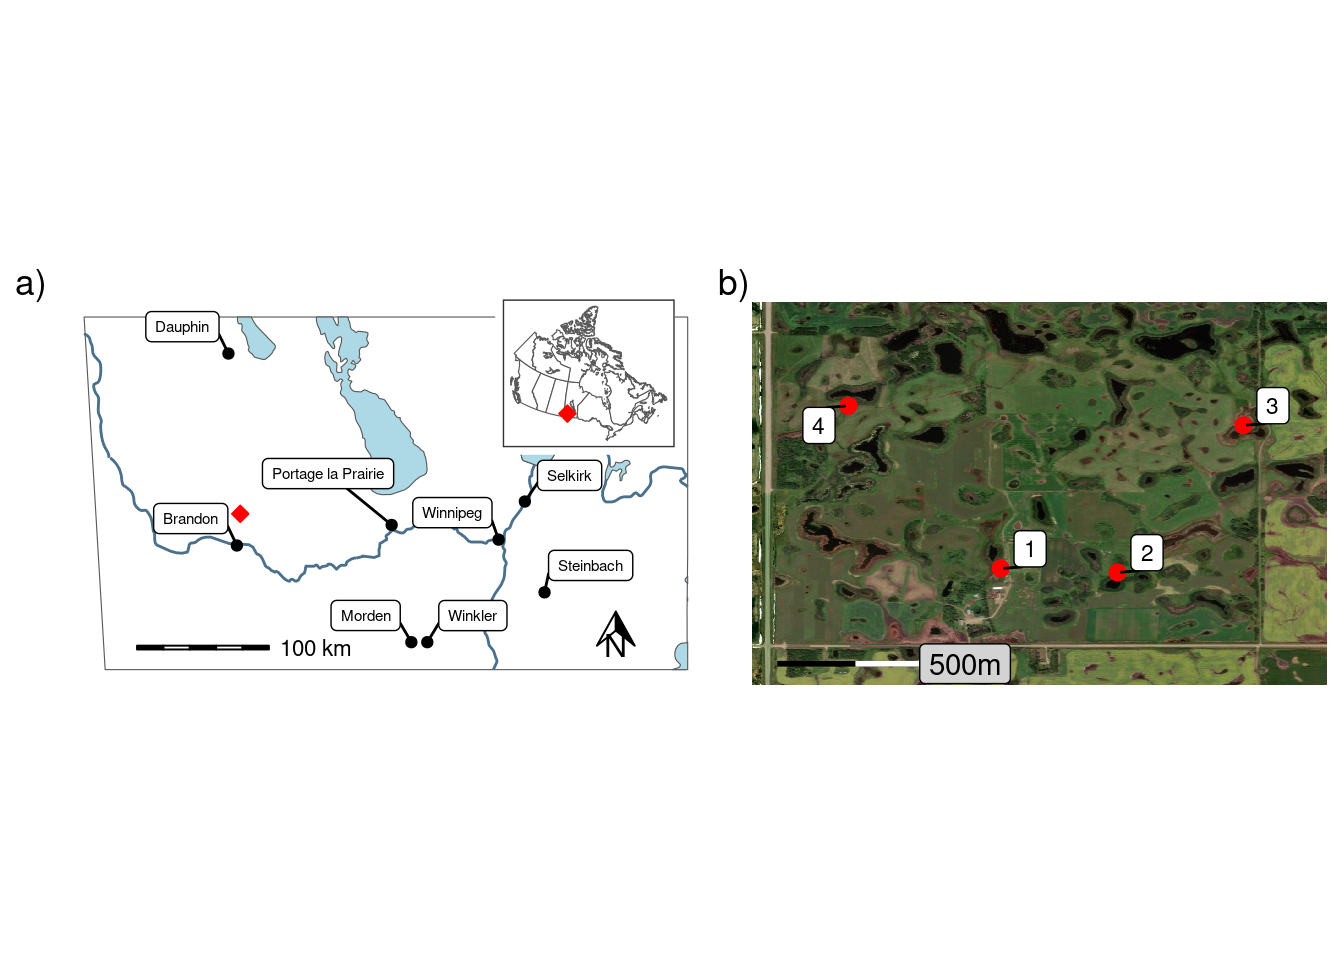
\includegraphics[keepaspectratio]{index_files/figure-latex/notebooks-05_Map-fig-mapr-output-2.png}}

}

\caption{\label{fig-mapr}Showing a) the location of the study site in
southern Manitoba with an inset map of Canada; and b) the locations of
the four riparian areas included in this study}

\end{figure}%

\textsubscript{Source:
\href{https://alex-koiter.github.io/riparian-grazing-manuscript/notebooks/05_Map-preview.html\#cell-fig-mapr}{Map
of study area}}

\subsection{Experimental design}\label{experimental-design}

Four riparian areas surrounding permanent wetlands were selected
(Figure~\ref{fig-mapr}) and subdivided into four approximately 450
\(m^2\) plots. Within each riparian area, each plot was randomly
assigned to a treatment or control. The experimental groups (i.e.,
treatments) were 1) control, 2) graze, 3) high-density graze, and 4) mow
and harvest. The grazing treatments consisted of a single five-hour
grazing period, with the grazing treatment having 3.1-3.5 animal units
per plot and the high-density grazing having 11.75-12 animal units.
These stocking densities were used to approximate a typical rotational
grazing and a mob grazing approach. The grazed plots were fenced on all
four sides, including the edge of the waterbody and provided with
supplemental water. The cattle grazing treatments occurred over four
consecutive days where each day the graze and high-density graze
treatments were completed at a given riparian area. The cattle were
transported between the riparian areas by trailer and were placed in a
holding area while not grazing the experimental plots. For the mowing
treatment, the vegetation was cut to a height of 10cm, and the
vegetation was manually raked out of the plot. Treatments were applied
early to mid-September, before the first frost, in three consecutive
years (2019-2021) (\quartosuppfigref{suppfig-weather-plot}). Within each
plot three distinctive sampling locations, or topographic positions,
were established, adjacent to the edge of the waterbody (lower),
adjacent to the field/pasture (upper), and at the mid-point (middle).
Samples were collected at each sampling location 1-3 days before and 1-3
days after treatment (including the control) to assess the impact of
grazing and mowing. Before and after samples were collected at
immediately adjacent locations.

\subsection{Sampling and analysis}\label{sampling-and-analysis}

Four types of samples were collected: 1) biomass, 2) litter, 3) organic
layer, and 4) Ah horizon. Using a 0.25 \(m^2\) quadrate, biomass was
collected by cutting the standing live vegetation and litter by raking
the surface and picking up the previous year's growth. Both the biomass
and litter were dried at 40 \(^\circ C\), weighed, and homogenized using
a blade grinder (\textless1cm). A composite of five soil samples was
collected within the same quadrat as the biomass/litter using a 19 mm
diameter soil probe and was divided into the organic layer (1 -- 2 cm
deep) and the top 10 cm of the Ah horizon. The organic layer and Ah soil
were air-dried, disaggregated with a mortar and pestle, and passed
through a 2-mm sieve. Additional bulk density samples of both the
organic layer and Ah and the depth of the organic layer were collected
in 2023. Daily air temperature and rainfall data were collected from an
onsite station (\quartosuppfigref{suppfig-weather-plot}) (Manitoba
Agriculture, 2023).

Water Extractable Phosphorus (WEP), an environmental soil and vegetation
P test, was used to infer soil P release into runoff water. Dried and
homogenized samples were extracted by shaking (150 RPM) with deionized
water for one hour at a mass-to-volume ratio of 1:30 for the biomass and
litter samples (1 g) and 1:15 for the organic and Ah samples (2 g).
Extractions were gravity filtered through a Whatman 42 filter followed
by syringe filtration with a 0.45 \(\mu m\) nylon filter. WEP in the
extract was measured spectrophotometrically by the colorimetric
molybdate--ascorbic acid method (Murphy and Riley, 1962; Sharpley et
al., 2006).

The concentration of WEP (\(mg~kg^{-1}\)) was calculated for all sources
of P. In addition, the areal density of WEP was calculated for biomass
and litter by combining WEP concentration with the mass of material
collected from the quadrat. The vertical profile of WEP within the
riparian area assessed from samples collected before treatments were
implemented across the 3-year study. For comparison, an approximate
estimation of areal density WEP in the organic layer and Ah was
calculated using the bulk density and depth measurements collected in
2023 (Figure~\ref{fig-vertical-wep} b).

\subsection{Statistical analysis}\label{statistical-analysis}

All statistical analysis, plotting, and mapping were undertaken using
the R Statistical Software (v4.4.1; R Core Team (2024)), through the
RStudio Integrated Development Environment v2023.12.1.402 (RStudio,
2024). All plots and maps were created using the R package
\texttt{ggplot2} (v3.5.1; Wickham (2016)). Country and regional maps
were created using data from the \texttt{rnaturalearth} package
(Massicotte and South, 2023) and other maps using ESRI imagery and the
\texttt{OpenStreetMap} package (Fellows, 2023). Four Linear Mixed Models
(R package \texttt{glmmTMB} v1.1.10; Brooks et al. (2017)) were used to
investigate the effect of treatment and riparian sampling location
(including interaction) on the numeric difference in WEP measurements
taken before and after treatment for each of the four distinct sources
of P (areal densities for biomass and litter; concentrations for organic
matter and Ah). Year and riparian area were included as crossed random
factors to control for the variability within years and riparian areas.

Additionally, when investigating the net change in biomass WEP the
initial biomass WEP (before applying the treatment) was included in the
model as a covariate. This controls for the fact that the magnitude of
the difference in biomass measurements taken before and after treatment
is directly related to the mass of WEP initially available. By
controlling for this, the model indicates which treatments resulted in a
relatively greater change in biomass, rather than simply absolute
change.

The interaction between treatment and riparian sampling location was
removed if non-significant (p \textless{} 0.05). When a main effect or
interaction was significant, post-hoc pairwise comparisons with a
Benjamini-Hochberg p-value adjustment were performed (p \textless0.05).
When a main effect or interaction was significant, post-hoc pairwise
comparisons with a Benjamini-Hochberg p-value adjustment was used
(\texttt{emmeans} v1.10.5; Lenth (2024)). Model assumptions were
assessed using DHARMa residual plots (\texttt{DHARMa} v0.4.6; Hartig
(2022)), main effects were tested for collinearity (\texttt{performance}
v0.12.4; Lüdecke et al. (2021)), and results were presented as type III
ANOVA (\texttt{car} v3.1.3; Fox and Weisberg (2019)). For each unique
source of WEP, the null hypotheses were 1) no difference in the net WEP
among treatments or riparian sampling locations and 2) no interactions
between these two factors.

Pearson correlations were performed to explore relations in WEP
concentrations among the four unique P sources for each of the three
topographic positions using samples collected before the application of
the treatments. These relations were visualized using a scatterplot
matrix created using the \texttt{GGally} R package (v2.2.1; Schloerke et
al. (2024) )

\section{Results and Discussion}\label{results-and-discussion}

\subsection{Vertical profiles of P}\label{vertical-profiles-of-p}

The biomass, litter, organic layer, and Ah horizon sources of P
demonstrated a strong vertical stratification in both the concentration
and areal densities of WEP (Figure~\ref{fig-vertical-wep}). The median
concentrations in the vegetation sources were 82.8 and 39.0
\(mg~kg^{-1}\) for the biomass and litter components, respectively,
which is more than an order of magnitude greater than the soil
components (0.9 and 3.4 \(mg~kg^{-1}\); Ah and organic, respectively).
Considerable variability in the WEP concentration in the biomass and
litter sources were observed with interquartile ranges (IQR) of 54.3 and
32.9 \(mg~kg^{-1}\) for the biomass and litter sources, respectively. In
contrast, the IQR for the organic and Ah sources both were \textless2.5
\(mg~kg^{-1}\).

Overall, in terms of the areal density of WEP, the top 10 cm of the Ah
horizon was the largest source of WEP (42.5 \(mg~m^{-2}\)) followed by
the biomass (26.3 \(mg~m^{-2}\)), organic layer (14.3 \(mg~m^{-2}\)),
and the litter (13.7 \(mg~m^{-2}\)). It should be noted that these are
only approximate estimates for the organic layer and Ah horizon because
the values for depth and bulk density measured in 2023 were used in the
calculations for all previous years. Nevertheless, the vertical profile
of WEP in riparian areas (Figure~\ref{fig-vertical-wep}) observed in
this study supports the concept that a measure of P in soil alone is
likely missing a large proportion of the near-surface P that can be
potentially lost during the spring snowmelt (Liu et al., 2019a; b; Cober
et al., 2019). The substantial proportion of WEP above the soil surface
provides evidence that managing the biomass in riparian areas in autumn
may reduce the contribution of P lost directly from this area during
spring. Specifically, the harvesting of this biomass results in an
export of P which can maintain or enhance the buffering or storage
capacity of P derived from upslope sources further improving downstream
water quality (Kelly et al., 2007; Hille et al., 2019).

\begin{figure}[H]

\centering{

\pandocbounded{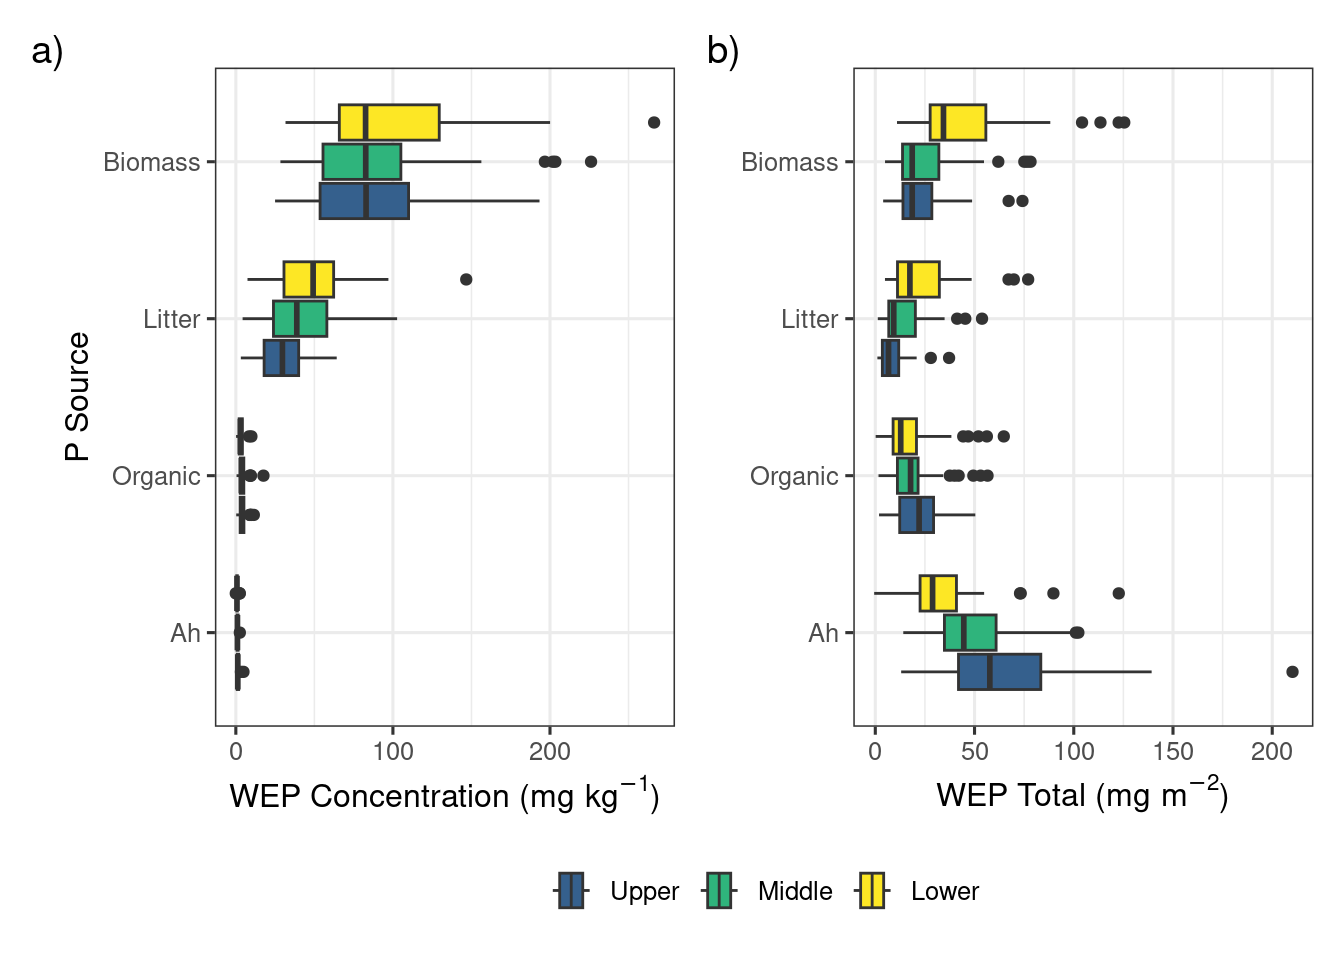
\includegraphics[keepaspectratio]{index_files/figure-latex/notebooks-04_Vertical_profile-fig-vertical-wep-output-2.png}}

}

\caption{\label{fig-vertical-wep}Vertical and longitudinal profiles of
a) WEP concentration and b) WEP content in the riparian areas prior to
grazing and mowing treatments.}

\end{figure}%

\textsubscript{Source:
\href{https://alex-koiter.github.io/riparian-grazing-manuscript/notebooks/04_Vertical_profile-preview.html\#cell-fig-vertical-WEP}{Vertical
profile of WEP}}

\subsection{Longitudinal profiles of
P}\label{longitudinal-profiles-of-p}

Prior to grazing and mowing treatments, the median WEP concentrations
were similar among the upper, mid, and lower positions for the biomass
samples. There was a small topographic trend in the WEP concentration
for both the Ah and organic litter P sources where the concentration
decreased from the upper through to the lower sampling locations. The
WEP concentrations in the Ah and organic layer were found to be
significantly (p \textless{} 0.001) and positively correlated
(r\textsuperscript{2} = 0.40) (Figure~\ref{fig-vertical-wep} and
\quartosuppfigref{suppfig-pairs-plot}). This topographic pattern is
consistent with other studies and is likely due to the rapid physical
and geochemical retention of upslope derived P within the first 5 m of
the riparian area (Syversen and Borch, 2005).The litter showed the
opposite topographic trend with higher WEP concentrations in the lower
sampling locations. There was a significant (p \textless{} 0.001)
positive correlation (r\textsuperscript{2} = 0.34)between the WEP
concentration in the biomass and litter samples suggesting that biomass
with a high WEP concentration produces litter with a high WEP
concentration (\quartosuppfigref{suppfig-pairs-plot}). There was no
correlation (p \textgreater{} 0.05) between the Ah and biomass WEP
concentrations suggesting that higher soil WEP concentration does not
result in biomass with elevated WEP concentrations at this study site
(\quartosuppfigref{suppfig-pairs-plot}). There is some evidence that
plants growing in P-rich environments can become enriched in P (e.g.,
Kröger et al., 2007); however, there was no correlation (p
\textgreater{} 0.05) between the Ah and biomass WEP concentrations
suggesting that higher soil WEP concentration does not result in biomass
with elevated WEP concentrations at this study site
(\quartosuppfigref{suppfig-pairs-plot}).

For the biomass and litter sources, the lower riparian locations had
greater areal densities of WEP whereas the organic and Ah sources had
greater areal densities of WEP in the upper riparian locations. The
longitudinal gradient of WEP showed an inverted symmetry where the
biomass WEP was largest near the lower sampling location and the Ah soil
WEP was largest in the upper sampling location adjacent to the fields
(Figure~\ref{fig-vertical-wep} b). The high soil water content in the
lower location created conditions that favor high biomass production
(\quartosuppfigref{suppfig-bd-plot}) ) and higher WEP concentration
(Figure~\ref{fig-vertical-wep} a). The higher bulk density was most
likely due to the lower soil organic matter content and the higher WEP
concentration may be related to the interception of P-rich runoff from
upslope areas (Tomer et al., 2007). Understanding and quantifying the
sources and patterns of P within riparian areas is a key part of
assessing the risk of P loss as it helps to inform management decisions
and target the largest sources of P (Reid et al., 2018).

\subsection{Impacts of grazing and mowing on P
sources}\label{impacts-of-grazing-and-mowing-on-p-sources}

There was considerable variation across all treatments and riparian
locations in all four P sources. This high variability in WEP areal
density/concentration is best reflected in the control treatment where
the expected difference was 0 (Figures 3 through 6), but WEP losses and
gains were still observed despite no treatment being applied. . For
example, the control plots had a median biomass WEP removal rate of 5.5
\(mg~m^{-2}\) (Figure~\ref{fig-vegetation-wep} a). However, despite this
variability, several patterns demonstrating relationships among
treatments and vertical and longitudinal P emerged.

Results of the linear mixed model of areal density of biomass WEP show a
significant effect of treatment (X\textsuperscript{2} = 24.8, df = 3, p
\textless{} 0.001) and riparian location (X\textsuperscript{2} = 15.7,
df = 2, p \textless{} 0.001). Post-hoc comparisons showed that the net
biomass WEP for the high-density grazing and mowing treatments were
similar (p\textgreater0.05) but significantly (p\textless0.05) different
from the control and graze treatments (Figure~\ref{fig-vegetation-wep} a
and Table~\ref{tbl-biomass-posthoc}).The mowing and high-density grazing
reduced the average WEP areal density by 7.4 and 4.2 \(mg~m^{-2}\)
relative to the control, respectively. The reduction in biomass WEP was
significantly (p\textless0.05) greater in the lower sampling locations
as compared to the upper and mid locations
(Figure~\ref{fig-vegetation-wep} b and Table~\ref{tbl-biomass-posthoc})
with a difference in average WEP of 10.2 \(mg~m^{-2}\) between the lower
and upper locations of the riparian area.

\begin{figure}[H]

\centering{

\pandocbounded{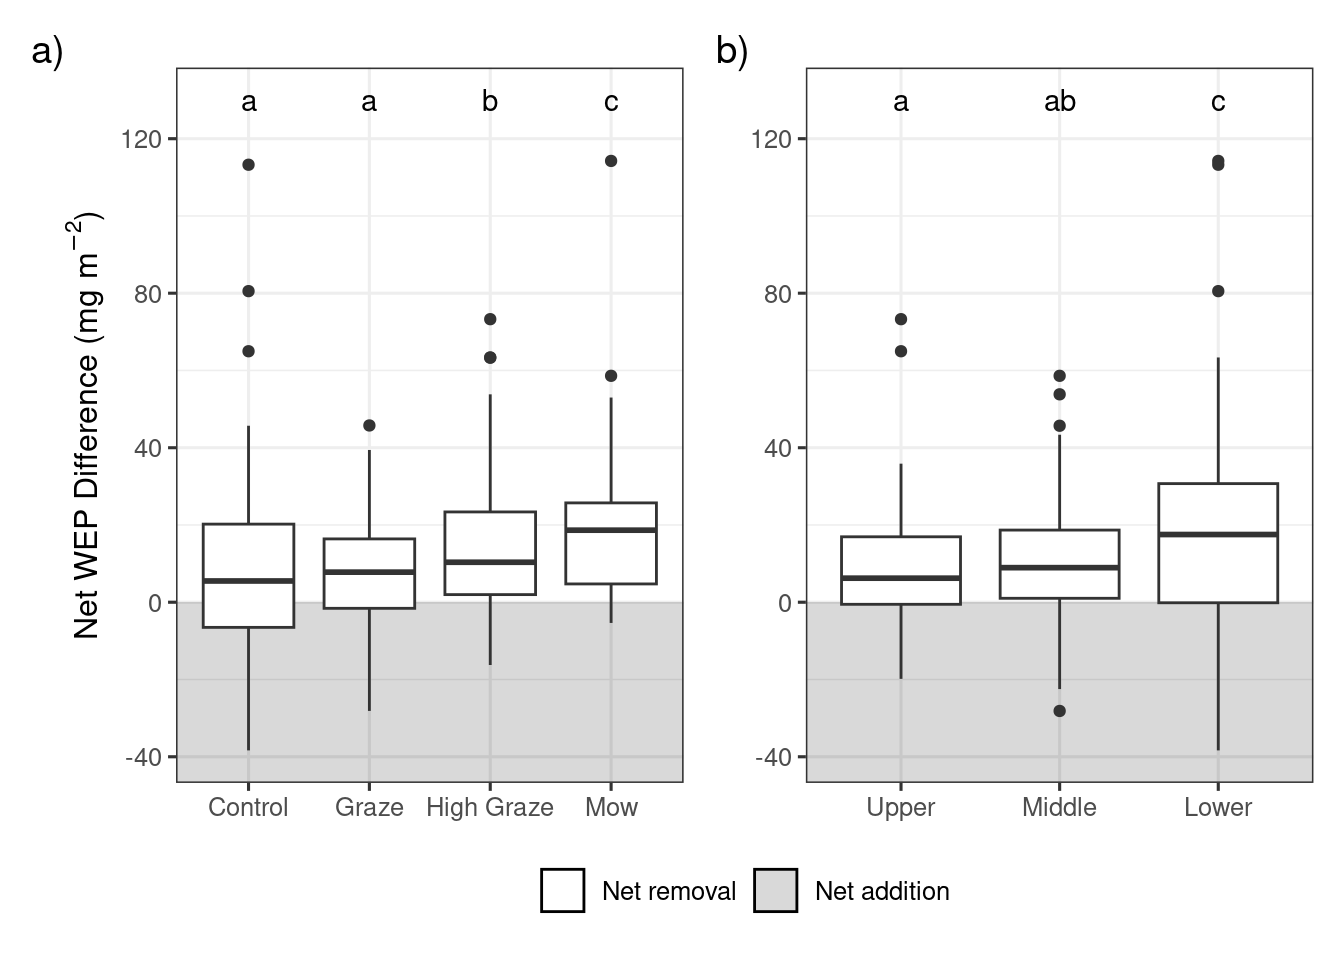
\includegraphics[keepaspectratio]{index_files/figure-latex/notebooks-01_Biomass_analysis-fig-vegetation-wep-output-2.png}}

}

\caption{\label{fig-vegetation-wep}Change in riparian biomass WEP
following grazing or mowing in each riparian location. Within each plot
significant differences (p\textless0.05) between treatments or riparian
locations are denoted with different letters. Lower sampling locations
are adjacent to the edge of the waterbody and Upper locations are
adjacent to the field.}

\end{figure}%

\textsubscript{Source:
\href{https://alex-koiter.github.io/riparian-grazing-manuscript/notebooks/01_Biomass_analysis-preview.html\#cell-fig-vegetation-WEP}{Riparian
vegetation WEP in response to grazing}}

\begin{longtable}[]{@{}cccccc@{}}

\caption{\label{tbl-biomass-posthoc}Results of the post-hoc pairwise
comparisons with a Benjamini-Hochberg p value adjustment for differences
in the net biomass WEP (\(mg~m^{-2}\)) between the four treatments and
three riparian sampling locations.}

\tabularnewline

\toprule\noalign{}
Contrast & Estimate & SE & df & t ratio & p value \\
\midrule\noalign{}
\endhead
\bottomrule\noalign{}
\endlastfoot
\multicolumn{6}{@{}c@{}}{%
Treatment} \\
Control - High Graze & −4.83 & 2.42 & 132 & −2.00 & 0.072 \\
Control - Mow & −8.52 & 2.42 & 132 & −3.52 & 0.002 \\
Control - Graze & 2.47 & 2.40 & 132 & 1.03 & 0.306 \\
High Graze - Mow & −3.69 & 2.43 & 132 & −1.51 & 0.159 \\
High Graze - Graze & 7.30 & 2.42 & 132 & 3.02 & 0.006 \\
Mow - Graze & 10.99 & 2.42 & 132 & 4.55 & \textless0.001 \\
\multicolumn{6}{@{}c@{}}{%
Location} \\
Lower - Middle & −7.94 & 2.43 & 132 & −3.26 & 0.002 \\
Lower - Upper & −9.82 & 2.57 & 132 & −3.83 & \textless0.001 \\
Middle - Upper & −1.87 & 2.11 & 132 & −0.89 & 0.377 \\

\end{longtable}

\textsubscript{Source:
\href{https://alex-koiter.github.io/riparian-grazing-manuscript/notebooks/01_Biomass_analysis-preview.html\#cell-tbl-biomass-posthoc}{Riparian
vegetation WEP in response to grazing}}

The model looking at areal density of litter WEP showed no significant
impacts of either treatment (X\textsuperscript{2} = 1.15, df = 3, p =
0.23) or riparian location (X\textsuperscript{2} = 4.30, df = 2, p =
0.56) (Figure~\ref{fig-litter-wep}). ). In contrast, the model exploring
WEP concentration in the organic layer detected no significant
difference among riparian locations (X\textsuperscript{2} = 0.57, df =
2, p = 0.75) but did find a significant effect of treatment
(X\textsuperscript{2} = 8.24, df = 3, p = 0.04). However, the post-hoc
pairwise comparisons (Table~\ref{tbl-organic-posthoc}) found no
significant differences (p \textless{} 0.05) among the treatments.
Finally, there was no significant effect of treatment
(X\textsuperscript{2} = 2.59, df = 3, p = 0.46) or riparian position
(X\textsuperscript{2} = 1.17, df = 2, p = 0.56) on the concentration of
WEP in the Ah horizon (Figure~\ref{fig-soil-wep}).

\begin{figure}[H]

\centering{

\pandocbounded{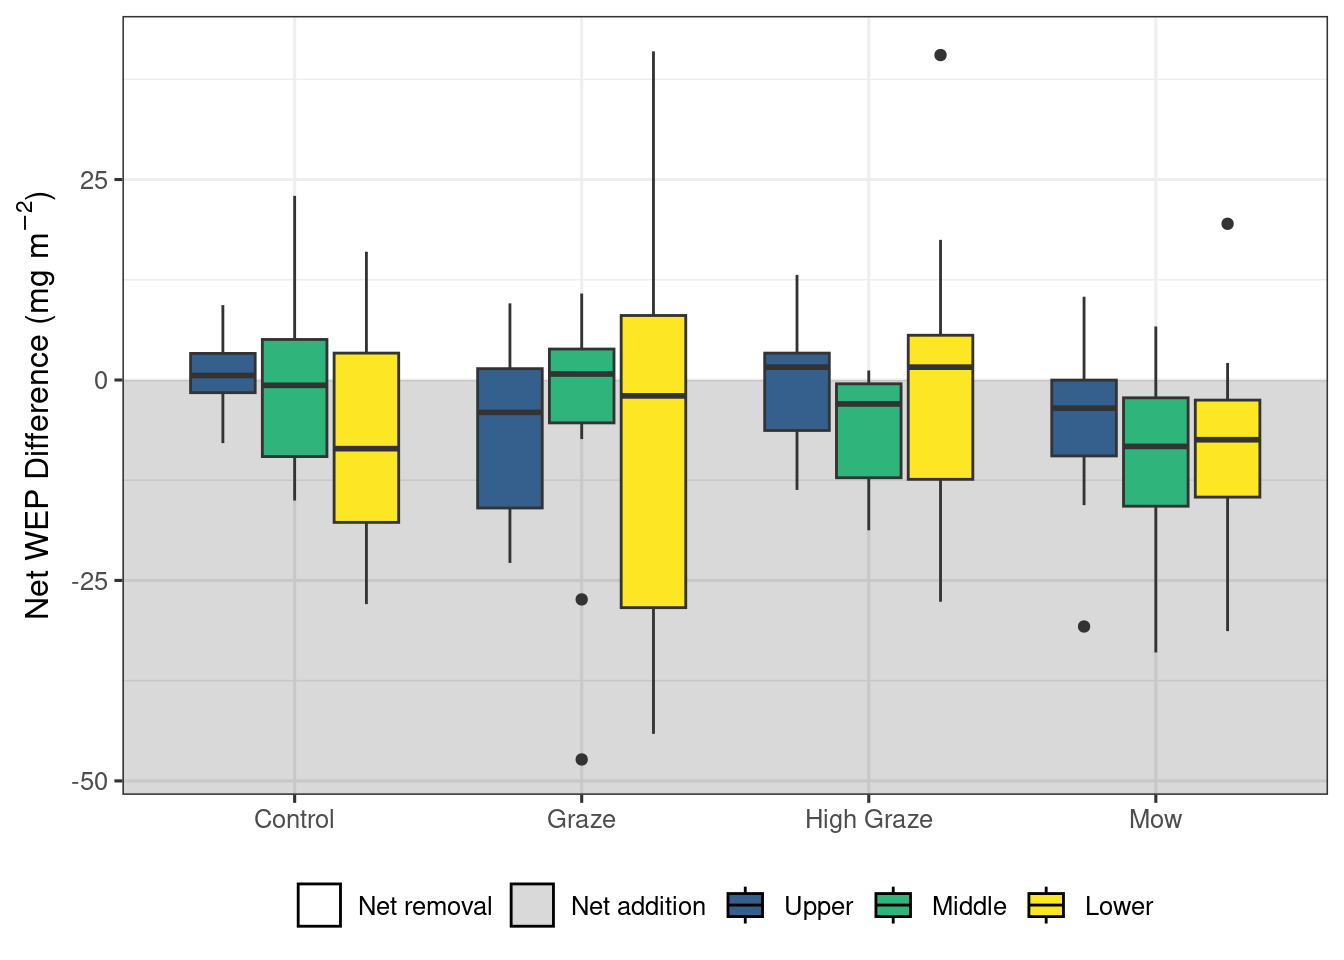
\includegraphics[keepaspectratio]{index_files/figure-latex/notebooks-02_Litter_analysis-fig-litter-wep-output-2.png}}

}

\caption{\label{fig-litter-wep}Change in riparian litter WEP following
grazing or mowing in each of the riparian locations. No significant
effect of treatment or riparian location on the litter WEP content was
detected. Lower sampling locations are adjacent to the edge of the
waterbody and Upper locations are adjacent to the field.}

\end{figure}%

\textsubscript{Source:
\href{https://alex-koiter.github.io/riparian-grazing-manuscript/notebooks/02_Litter_analysis-preview.html\#cell-fig-litter-WEP}{Riparian
litter WEP in response to grazing}}

\begin{figure}[H]

\centering{

\pandocbounded{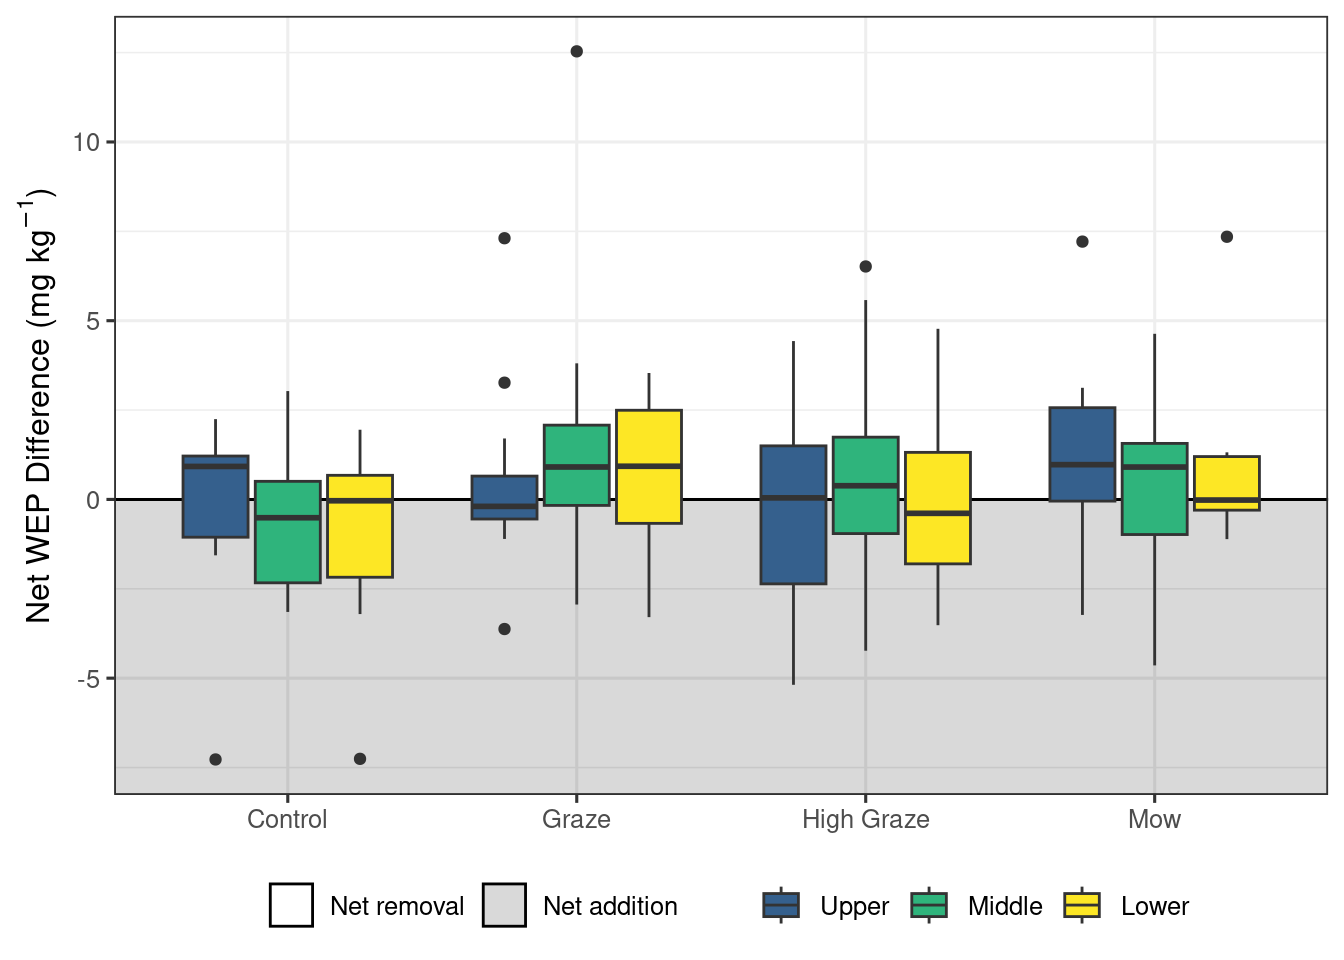
\includegraphics[keepaspectratio]{index_files/figure-latex/notebooks-03_Soils_analysis-fig-organic-wep-output-1.png}}

}

\caption{\label{fig-organic-wep}Change in riparian organic layer WEP
concentration following grazing or mowing in each of the riparian
locations. A significant effect of treatment was detected; however, the
post-hoc analysis was not able to detect any significant (p \textless{}
0.05) pairwise contrasts. Lower sampling locations are adjacent to the
edge of the waterbody and Upper locations are adjacent to the field.}

\end{figure}%

\textsubscript{Source:
\href{https://alex-koiter.github.io/riparian-grazing-manuscript/notebooks/03_Soils_analysis-preview.html\#cell-fig-organic-WEP}{Riparian
organic and mineral soil WEP in response to grazing}}

\begin{longtable}[]{@{}llllll@{}}

\caption{\label{tbl-organic-posthoc}Results of the post-hoc pairwise
comparisons with a Benjamini-Hochberg p value adjustment for differences
in the net organic layer WEP (\(mg~kg^{-1}\)) between the four
treatments.}

\tabularnewline

\toprule\noalign{}
Contrast & Estimate & SE & df & t ratio & p value \\
\midrule\noalign{}
\endhead
\bottomrule\noalign{}
\endlastfoot
Control - Graze & −1.49 & 0.59 & 135 & −2.50 & 0.066 \\
Control - High Graze & −0.63 & 0.59 & 135 & −1.05 & 0.353 \\
Control - Mow & −1.38 & 0.59 & 135 & −2.32 & 0.066 \\
Graze - High Graze & 0.86 & 0.59 & 135 & 1.45 & 0.299 \\
Graze - Mow & 0.11 & 0.59 & 135 & 0.18 & 0.856 \\
High Graze - Mow & −0.75 & 0.59 & 135 & −1.27 & 0.311 \\

\end{longtable}

\textsubscript{Source:
\href{https://alex-koiter.github.io/riparian-grazing-manuscript/notebooks/03_Soils_analysis-preview.html\#cell-tbl-organic-posthoc}{Riparian
organic and mineral soil WEP in response to grazing}}

\begin{figure}[H]

\centering{

\pandocbounded{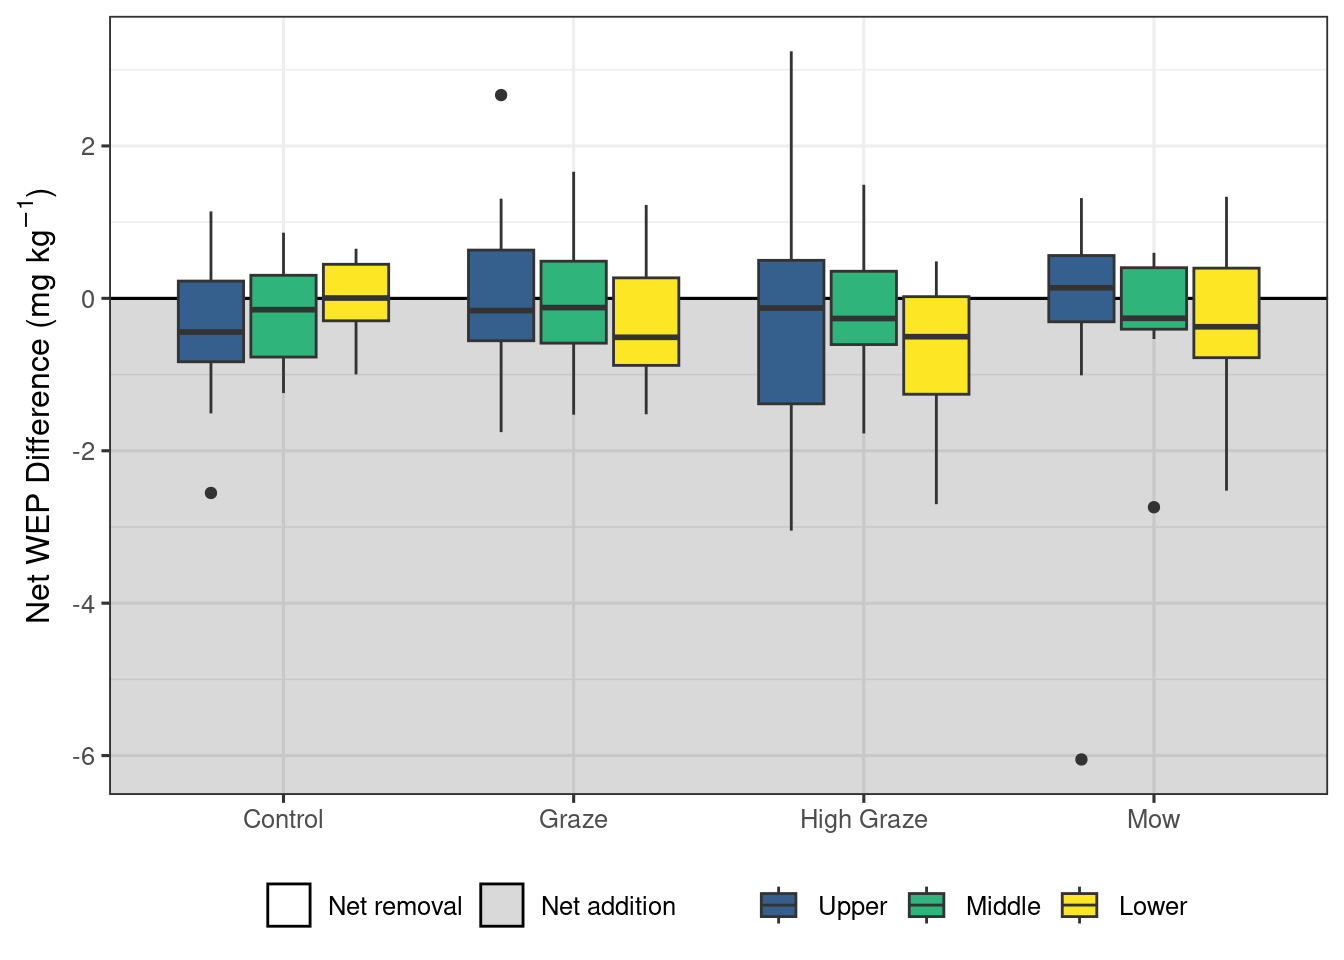
\includegraphics[keepaspectratio]{index_files/figure-latex/notebooks-03_Soils_analysis-fig-soil-wep-output-1.png}}

}

\caption{\label{fig-soil-wep}Change in riparian Ah layer (0-10cm) WEP
concentration following grazing or mowing in each of the riparian
locations. No significant effect of treatment or location was detected.
Lower sampling locations are adjacent to the edge of the waterbody and
Upper locations are adjacent to the field.}

\end{figure}%

\textsubscript{Source:
\href{https://alex-koiter.github.io/riparian-grazing-manuscript/notebooks/03_Soils_analysis-preview.html\#cell-fig-soil-WEP}{Riparian
organic and mineral soil WEP in response to grazing}}

Taken together, these results suggest that short-term autumn
high-density grazing may be a potential management tool that can reduce
the mass of P lost directly from the riparian area
(Figure~\ref{fig-vegetation-wep} a). In addition to managing P loss,
grazing riparian areas can also provide an essential source of forage,
particularly during drought. Mechanized harvesting of biomass could also
achieve this reduction in P loss (Figure~\ref{fig-vegetation-wep} a) if
the landscape and soil conditions are favorable. Despite the cycling of
nutrients by the removal of P through grazing of biomass
(Figure~\ref{fig-vegetation-wep}) and the deposition through excretion,
no differences were detected in the litter and Ah sources of P
(Figure~\ref{fig-litter-wep}, and \ref{fig-soil-wep}). The models did
detect a significant effect of treatment on the organic layer WEP;
however, the pairwise comparisons were not able to detect any
significant differences and the exact nature of the impact of the
treatments remains unclear.

The ability to detect changes in the WEP sources in riparian areas is
difficult due to spatial variability in both the pre- and post-grazing
treatments. Even within the control plots, both net addition and removal
of WEP were detected and in many cases the variability was similar to
the other treatments. This inherent variability (i.e., pre-grazing)
likely results from a combination of hydrological factors like ground
water fluctuations, soil attributes such as texture, ecological dynamics
involving plant community composition, and anthropogenic influences like
historical land management practices (McClain et al., 2003; Vidon et
al., 2010). In particular, the species cover information
(\quartosuppfigref{suppfig-plant-plot}) demonstrates a wide range in
species composition and abundance, this coupled with the variation in P
release with different vegetation species may explain some of the
observed variability (Cober et al., 2018).

\subsection{Sources of variability and uncertainty in P
sources}\label{sources-of-variability-and-uncertainty-in-p-sources}

The prairie pothole wetlands regularly experience high water levels in
the early spring. Automated observations made with a water level logger
adjacent to one plot between October 2020 and May 2021 showed that the
lower, middle, and upper sampling points experienced inundation for
approximately 21, 11, and zero days, respectively (Noyes et al., 2024).
The annual weather conditions and topography of riparian areas
surrounding the wetlands will impact the length and extent of flooding.
Prolonged contact with water has been shown to increase the mass of WEP
lost in both soil (Young and Briggs, 2008) and vegetation (Lozier and
Macrae, 2017) and may also explain some of the observed variability. As
reported by Podolsky and Schindler (1993), the soils surrounding these
potholes are typically low in CaCo\textsubscript{3} and have a neutral
to slight alkaline pH. In this pH range (6.5 to 7.5) P availability is
typically at its highest and not expected to precipitate with Ca. A more
detailed soil chemical analysis, particularly Fe and Mn, along with soil
saturation duration information (i.e., redox) would be needed to fully
assess the potential for P loss during the spring (Walton et al., 2020).

The WEP protocol used for both soil and vegetation samples are not
likely to capture redox-sensitive mobilized P from the soil (Walton et
al., 2020) or enhanced P leaching from vegetation (Lozier and Macrae,
2017). Similarly, the WEP protocol also does not capture the enhanced P
release from soil and vegetation that results repeated freeze-thaw
cycles (Liu et al., 2013; Lozier and Macrae, 2017). However, temperature
sensors placed at the soil surface adjacent to one plot recorded four
freeze-thaw cycles between Oct 2020 and May 2021 and found that surface
temperatures fluctuations are moderated in this region by the relatively
persistent snowpack (Noyes et al., 2024).), reducing the potential
effects of freeze-thaw cycles on P release. However, both the prolonged
contact with water and freeze-thaw cycles are not captured in the WEP
protocols and may result in an underestimation of the potential for P
loss from each of the four distinctive sources of P in riparian areas.

In addition to climatic effects, there may be variability in P as a side
effect of the study design. One source of variability could be from
added urine and manure in grazed areas which likely created additional
hotspots of P that may carry forward to subsequent years (Subedi et al.,
2020; Donohoe et al., 2021). However, there was no indication of P
accumulation due to grazing in any of the four distinctive P sources
over the 3-year study period. The highest concentrations of WEP were
typically found in the second year of the study
(\quartosuppfigref{suppfig-years-plot}). This suggests that other
biophysical processes regulated by weather conditions
(\quartosuppfigref{suppfig-weather-plot}) were of greater importance in
controlling the WEP concentrations than P additions from cattle urine
and manure.

Another source of variability may have been from sampling. As there was
significant variability among plots, the single 0.25 \(m^2\) sampling
quadrat within each riparian location may have been insufficient to
capture the spatial variability. Therefore, larger composite and/or
several sampling locations within each upper, middle and lower locations
are recommended. Appropriate sampling design becomes critical as the
scale of observation of similar research increases to the farm scale,
and so will the range and sources of variability. As the scope of
research is expanded to the farm level, the importance of using an
appropriate sampling design becomes increasingly critical (Hale et al.,
2014).

\subsection{Management implications}\label{management-implications}

Autumn was selected for the mowing and grazing treatments for three
reasons. The first was to reduce the mass of biomass P available that
can contribute to the P loss during the spring snowmelt. Second, drier
soil conditions reduce the extent of pugging and soil compaction, which
limits the disruption of soil structure and damage to plants (Batey,
2009). Lastly, the prairie potholes and associated riparian areas are
important breeding habitats for migratory birds. Grazing can negatively
affect these species, but late-season grazing may reduce this potential
ecological impact (Stanley and Knopf, 2002). However, the type of
grazing system (timing, stocking rate, and density, etc.) may impact
habitat quality and breeding success (Carnochan et al., 2018; Hansen et
al., 2019; Kraft et al., 2021).

Corridor fencing at the edge of the waterbody and alternative water
sources were used in this study to limit livestock access to prevent
bank erosion and protect water quality (e.g., direct deposition)
(Dauwalter et al., 2018). Scaling this to the farm level would require
virtual fencing or infrastructure (Aarons et al., 2013) and time (to
conduct short-term grazing), especially in prairie pothole region where
there are numerous and small riparian areas (Sovell et al., 2000;
Hubbard et al., 2004; Hulvey et al., 2021; Manitoba Agriculture, 2024).

The long-term impacts of repeated grazing of riparian areas also need to
be considered. From a nutrient loss reduction perspective, a shift in
the magnitude of P sources could be expected as less biomass is
available to be added to the litter source, affecting the organic layer
and Ah sources of P. The regular inclusion of cattle will also introduce
a new manure source of P, which can spatially redistribute P and
initially be more water soluble and readily transported (Franzluebbers
et al., 2019). Grazing can also reduce the litter layer through
trampling increasing the soil-vegetation contact and speeding up the
decomposition process. These changes in biomass and litter quantities
may result in changes to habitat structure. Although this study
generally considers environmental implications, forage management
practices also have an agronomic effect which should be taken into
consideration when developing best management practices (Subedi et al.,
2020).

\section{Conclusion}\label{conclusion}

Biomass and litter are significant sources of near-surface WEP in
riparian areas that have been historically disregarded in studies.
Management of the biomass prior to the onset of winter conditions in
cold climates has the potential to reduce the mass of P directly lost
during the spring snowmelt and maintain or enhance the nutrient
buffering capacity. The results from this experiment demonstrated that
short-term, high-density cattle grazing and mowing both resulted in a
reduction in the mass of biomass WEP, particularly in the lower riparian
locations. The grazing and mowing treatments had no detectable effect on
the other three near-surface sources of WEP. However, detecting changes
in the near-surface sources of WEP is challenging due to high spatial
variability.

Additional work on riparian management strategies is needed to address
the specific challenges posed by cold climates. In these regions, the
runoff and nutrient losses occur predominately during the spring
snowmelt period when the ability of riparian areas to trap and retain
nutrients is diminished. Further, the repeated freeze-thaw cycles of the
vegetation and soils increases the potential P losses during this key
time. Continued research to identify, quantify, and manage these sources
of P to improve water quality remains a priority. In addition to
improving water quality, the development of riparian management
strategies should prioritize the protection of other ecological goods
and services and recognize these areas as an integral part of the farm.

\section*{Acknowledgements}\label{acknowledgements}
\addcontentsline{toc}{section}{Acknowledgements}

This project was undertaken with the financial support of the Government
of Canada through the federal Department of Environment and Climate
Change and a Lake Winnipeg Basin Program grant awarded to the Manitoba
Association of Watersheds. Additional research funding was provided
through a Brandon University Research Committee grant awarded to AK.
Thank you to A. Avila, M. Luna, C Sobchuk, and A. Tan for all the help
with lab and field work. Special thanks to the Manitoba Beef and Forage
Initiatives research farm staff for the use of their facilities and
managing the cattle grazing and mowing treatments. Lastly, thank you to
R. Canart and M. Elsinger for helping to develop the experimental
design.

\section*{Data availability}\label{data-availability}
\addcontentsline{toc}{section}{Data availability}

Data and source code for analysis and manuscript available on GitHub:
\url{https://github.com/alex-koiter/riparian-grazing-manuscript}

\section*{Conflict of interest
statement}\label{conflict-of-interest-statement}
\addcontentsline{toc}{section}{Conflict of interest statement}

The authors have no competing interests to declare that are relevant to
the content of this article.

\section*{Author contributions}\label{author-contributions}
\addcontentsline{toc}{section}{Author contributions}

\textbf{A Koiter:} Conceptualization; Funding acquisition; Methodology
(equal); Investigation (equal); Data curation (equal); Formal analysis;
Visualization; Writing -- original draft (lead); writing -- review and
editing (lead). \textbf{T. Malone:} Methodology (equal); Data curation
(equal); Investigation (equal); Writing -- original draft (supporting);
Writing -- review and editing (supporting).

\section*{References}\label{references}
\addcontentsline{toc}{section}{References}

\phantomsection\label{refs}
\begin{CSLReferences}{1}{1}
\vspace{1em}

\bibitem[\citeproctext]{ref-aarons2013}
Aarons, S.R., A.R. Melland, and L. Dorling. 2013. Dairy farm impacts of
fencing riparian land: Pasture production and farm productivity. Journal
of Environmental Management 130: 255--266. doi:
\href{https://doi.org/10.1016/j.jenvman.2013.08.060}{10.1016/j.jenvman.2013.08.060}.

\bibitem[\citeproctext]{ref-batey2009}
Batey, Tom. 2009. Soil compaction and soil management {\textendash} a
review. Soil Use and Management 25(4): 335--345. doi:
\href{https://doi.org/10.1111/j.1475-2743.2009.00236.x}{10.1111/j.1475-2743.2009.00236.x}.

\bibitem[\citeproctext]{ref-beck2018}
Beck, H.E., N.E. Zimmermann, T.R. McVicar, N. Vergopolan, A. Berg, et
al. 2018. Present and future Köppen-Geiger climate classification maps
at 1-km resolution. Scientific Data 5(1): 180214. doi:
\href{https://doi.org/10.1038/sdata.2018.214}{10.1038/sdata.2018.214}.

\bibitem[\citeproctext]{ref-brooks2017}
Brooks, M.E., K. Kristensen, K.J. van Benthem, A. Magnusson, C.W. Berg,
et al. 2017. {glmmTMB} balances speed and flexibility among packages for
zero-inflated generalized linear mixed modeling. The R Journal 9(2):
378--400. doi:
\href{https://doi.org/10.32614/RJ-2017-066}{10.32614/RJ-2017-066}.

\bibitem[\citeproctext]{ref-carlyle2001}
Carlyle, G.C., and A.R. Hill. 2001. Groundwater phosphate dynamics in a
river riparian zone: Effects of hydrologic flowpaths, lithology and
redox chemistry. Journal of Hydrology 247(3): 151--168. doi:
\href{https://doi.org/10.1016/S0022-1694(01)00375-4}{10.1016/S0022-1694(01)00375-4}.

\bibitem[\citeproctext]{ref-carnochan2018}
Carnochan, S.J., C.C. De Ruyck, and N. Koper. 2018. Effects of
twice-over rotational grazing on songbird nesting success in years with
and without flooding. Rangeland Ecology \& Management 71(6): 776--782.
doi:
\href{https://doi.org/10.1016/j.rama.2018.04.013}{10.1016/j.rama.2018.04.013}.

\bibitem[\citeproctext]{ref-cober2018}
Cober, J.R., M.L. Macrae, and L.L. Van Eerd. 2018. Nutrient release from
living and terminated cover crops under variable freeze{\textendash}thaw
cycles. Agronomy Journal 110(3): 1036--1045. doi:
\href{https://doi.org/10.2134/agronj2017.08.0449}{10.2134/agronj2017.08.0449}.

\bibitem[\citeproctext]{ref-cober2019}
Cober, J.R., M.L. Macrae, and L.L. Van Eerd. 2019. Winter phosphorus
release from cover crops and linkages with runoff chemistry. Journal of
Environmental Quality 48(4): 907--914. doi:
\href{https://doi.org/10.2134/jeq2018.08.0307}{10.2134/jeq2018.08.0307}.

\bibitem[\citeproctext]{ref-dauwalter2018}
Dauwalter, D.C., K.A. Fesenmyer, S.W. Miller, and T. Porter. 2018.
Response of riparian vegetation, instream habitat, and aquatic biota to
riparian grazing exclosures. North American Journal of Fisheries
Management 38(5): 1187--1200. doi:
\href{https://doi.org/10.1002/nafm.10224}{10.1002/nafm.10224}.

\bibitem[\citeproctext]{ref-donohoe2021}
Donohoe, G., D. Flaten, F. Omonijo, and K. Ominski. 2021. Short-term
impacts of winter bale grazing beef cows on forage production and soil
nutrient status in the eastern canadian prairies. Canadian Journal of
Soil Science 101(4): 717--733. doi:
\href{https://doi.org/10.1139/cjss-2021-0028}{10.1139/cjss-2021-0028}.

\bibitem[\citeproctext]{ref-environmentandclimatechangecanada2024}
Environment, and Climate Change Canada. 2024. Canadian Climate Normals.
\url{https://climate.weather.gc.ca/climate_normals/index_e.html}.

\bibitem[\citeproctext]{ref-fellows2023}
Fellows, I. 2023.
\href{https://CRAN.R-project.org/package=OpenStreetMap}{OpenStreetMap:
Access to open street map raster images}.

\bibitem[\citeproctext]{ref-fitch2003}
Fitch, L., B. Adams, and K. O'Shaughnessy. 2003. Caring for the green
zone: Riparian areas and grazing management. 3rd ed. Cows; Fish Program,
Lethbridge, Alberta.

\bibitem[\citeproctext]{ref-fox2019}
Fox, J., and S. Weisberg. 2019.
\href{https://socialsciences.mcmaster.ca/jfox/Books/Companion/}{An {R}
companion to applied regression}. Third. Sage, Thousand Oaks {CA}.

\bibitem[\citeproctext]{ref-franzluebbers2019}
Franzluebbers, A.J., M.H. Poore, S.R. Freeman, and J.R. Rogers. 2019.
Soil-surface nutrient distributions in grazed pastures of North
Carolina. Journal of Soil and Water Conservation 74(6): 571--583. doi:
\href{https://doi.org/10.2489/jswc.74.6.571}{10.2489/jswc.74.6.571}.

\bibitem[\citeproctext]{ref-habibiandehkordi2019}
Habibiandehkordi, R., D.A. Lobb, P.N. Owens, and D.N. Flaten. 2019.
Effectiveness of vegetated buffer strips in controlling legacy
phosphorus exports from agricultural land. Journal of Environmental
Quality 48(2): 314--321. doi:
\href{https://doi.org/10.2134/jeq2018.04.0129}{10.2134/jeq2018.04.0129}.

\bibitem[\citeproctext]{ref-habibiandehkordi2017}
Habibiandehkordi, R., D.A. Lobb, S.C. Sheppard, D.N. Flaten, and P.N.
Owens. 2017. Uncertainties in vegetated buffer strip function in
controlling phosphorus export from agricultural land in the canadian
prairies. Environmental Science and Pollution Research 24(22):
18372--18382. doi:
\href{https://doi.org/10.1007/s11356-017-9406-6}{10.1007/s11356-017-9406-6}.

\bibitem[\citeproctext]{ref-hale2014}
Hale, R., P. Reich, T. Daniel, P.S. Lake, and T.R. Cavagnaro. 2014.
Scales that matter: Guiding effective monitoring of soil properties in
restored riparian zones. Geoderma 228-229: 173--181. doi:
\href{https://doi.org/10.1016/j.geoderma.2013.09.019}{10.1016/j.geoderma.2013.09.019}.

\bibitem[\citeproctext]{ref-hansen2019}
Hansen, B.D., H.S. Fraser, and C.S. Jones. 2019. Livestock grazing
effects on riparian bird breeding behaviour in agricultural landscapes.
Agriculture, Ecosystems \& Environment 270-271: 93--102. doi:
\href{https://doi.org/10.1016/j.agee.2018.10.016}{10.1016/j.agee.2018.10.016}.

\bibitem[\citeproctext]{ref-hartig2022}
Hartig, F. 2022.
\href{https://CRAN.R-project.org/package=DHARMa}{DHARMa: Residual
diagnostics for hierarchical (multi-level / mixed) regression models}.

\bibitem[\citeproctext]{ref-hille2019}
Hille, S., D. Graeber, B. Kronvang, G.H. Rubæk, N. Onnen, et al. 2019.
Management options to reduce phosphorus leaching from vegetated buffer
strips. Journal of Environmental Quality 48(2): 322--329. doi:
\href{https://doi.org/10.2134/jeq2018.01.0042}{10.2134/jeq2018.01.0042}.

\bibitem[\citeproctext]{ref-hubbard2004}
Hubbard, R.K., G.L. Newton, and G.M. Hill. 2004. Water quality and the
grazing animal1. Journal of Animal Science 82(suppl{\_}13): E255--E263.
doi:
\href{https://doi.org/10.2527/2004.8213_supplE255x}{10.2527/2004.8213\_supplE255x}.

\bibitem[\citeproctext]{ref-hulvey2021}
Hulvey, K.B., C.D. Mellon, and A.R. Kleinhesselink. 2021. Rotational
grazing can mitigate ecosystem service trade-offs between livestock
production and water quality in semi-arid rangelands. Journal of Applied
Ecology 58(10): 2113--2123. doi:
\href{https://doi.org/10.1111/1365-2664.13954}{10.1111/1365-2664.13954}.

\bibitem[\citeproctext]{ref-kelly2007}
Kelly, J.M., J.L. Kovar, R. Sokolowsky, and T.B. Moorman. 2007.
Phosphorus uptake during four years by different vegetative cover types
in a riparian buffer. Nutrient Cycling in Agroecosystems 78(3):
239--251. doi:
\href{https://doi.org/10.1007/s10705-007-9088-4}{10.1007/s10705-007-9088-4}.

\bibitem[\citeproctext]{ref-kieta2019}
Kieta, K.A., and P.N. Owens. 2019. Phosphorus release from shoots of
phleum pretense l. After repeated freeze-thaw cycles and harvests.
Ecological Engineering 127: 204--211. doi:
\href{https://doi.org/10.1016/j.ecoleng.2018.11.024}{10.1016/j.ecoleng.2018.11.024}.

\bibitem[\citeproctext]{ref-kieta2018}
Kieta, K.A., P.N. Owens, D.A. Lobb, J.A. Vanrobaeys, and D.N. Flaten.
2018. Phosphorus dynamics in vegetated buffer strips in cold climates: A
review. Environmental Reviews 26(3): 255--272. doi:
\href{https://doi.org/10.1139/er-2017-0077}{10.1139/er-2017-0077}.

\bibitem[\citeproctext]{ref-kraft2021}
Kraft, J.D., D.A. Haukos, M.R. Bain, M.B. Rice, S. Robinson, et al.
2021. Using grazing to manage herbaceous structure for a
heterogeneity-dependent bird. The Journal of Wildlife Management 85(2):
354--368. doi:
\href{https://doi.org/10.1002/jwmg.21984}{10.1002/jwmg.21984}.

\bibitem[\citeproctext]{ref-krall2023}
Krall, M., and P. Roni. 2023. Effects of livestock exclusion on stream
habitat and aquatic biota: A review and recommendations for
implementation and monitoring. North American Journal of Fisheries
Management 43(2): 476--504. doi:
\href{https://doi.org/10.1002/nafm.10863}{10.1002/nafm.10863}.

\bibitem[\citeproctext]{ref-kruxf6ger2007}
Kröger, R., M.M. Holland, M.T. Moore, and C.M. Cooper. 2007. Plant
senescence: A mechanism for nutrient release in temperate agricultural
wetlands. Environmental Pollution 146(1): 114--119. doi:
\href{https://doi.org/10.1016/j.envpol.2006.06.005}{10.1016/j.envpol.2006.06.005}.

\bibitem[\citeproctext]{ref-lacas2005}
Lacas, J.-G., M. Voltz, V. Gouy, N. Carluer, and J.-J. Gril. 2005. Using
grassed strips to limit pesticide transfer to surface water: A review.
Agronomy for Sustainable Development 25(2): 253--266. doi:
\href{https://doi.org/10.1051/agro:2005001}{10.1051/agro:2005001}.

\bibitem[\citeproctext]{ref-lenth2024}
Lenth, R.V. 2024.
\href{https://CRAN.R-project.org/package=emmeans}{Emmeans: Estimated
marginal means, aka least-squares means}.

\bibitem[\citeproctext]{ref-liu2019}
Liu, J., H.M. Baulch, M.L. Macrae, H.F. Wilson, J.A. Elliott, et al.
2019a. Agricultural water quality in cold climates: processes, drivers,
management options, and research needs. Journal of Environmental Quality
48(4): 792--802. doi:
\href{https://doi.org/10.2134/jeq2019.05.0220}{10.2134/jeq2019.05.0220}.

\bibitem[\citeproctext]{ref-liu2013}
Liu, J., R. Khalaf, B. Ulén, and G. Bergkvist. 2013. Potential
phosphorus release from catch crop shoots and roots after
freezing-thawing. Plant and Soil 371(1): 543--557. doi:
\href{https://doi.org/10.1007/s11104-013-1716-y}{10.1007/s11104-013-1716-y}.

\bibitem[\citeproctext]{ref-liu2019a}
Liu, J., M.L. Macrae, J.A. Elliott, H.M. Baulch, H.F. Wilson, et al.
2019b. Impacts of cover crops and crop residues on phosphorus losses in
cold climates: a review. Journal of Environmental Quality 48(4):
850--868. doi:
\href{https://doi.org/10.2134/jeq2019.03.0119}{10.2134/jeq2019.03.0119}.

\bibitem[\citeproctext]{ref-lozier2017}
Lozier, T.M., and M.L. Macrae. 2017. Potential phosphorus mobilization
from above-soil winter vegetation assessed from laboratory water
extractions following freeze{\textendash}thaw cycles. Canadian Water
Resources Journal 42(3): 276--288. doi:
\href{https://doi.org/10.1080/07011784.2017.1331140}{10.1080/07011784.2017.1331140}.

\bibitem[\citeproctext]{ref-ludecke2021}
Lüdecke, D., M.S. Ben-Shachar, I. Patil, P. Waggoner, and D. Makowski.
2021. {performance}: An {R} package for assessment, comparison and
testing of statistical models. Journal of Open Source Software 6(60):
3139. doi:
\href{https://doi.org/10.21105/joss.03139}{10.21105/joss.03139}.

\bibitem[\citeproctext]{ref-lyu2021}
Lyu, C., X. Li, P. Yuan, Y. Song, H. Gao, et al. 2021. Nitrogen
retention effect of riparian zones in agricultural areas: A
meta-analysis. Journal of Cleaner Production 315: 128143. doi:
\href{https://doi.org/10.1016/j.jclepro.2021.128143}{10.1016/j.jclepro.2021.128143}.

\bibitem[\citeproctext]{ref-manitobaagriculture2023}
Manitoba Agriculture. 2023. Manitoba agriculture weather program.
\url{https://www.gov.mb.ca/agriculture/weather/manitoba-ag-weather.html}.

\bibitem[\citeproctext]{ref-manitobaagriculture2024}
Manitoba Agriculture. 2024. Agriculture rotational grazing.
\url{https://www.gov.mb.ca/agriculture/}.

\bibitem[\citeproctext]{ref-manitobabeefforageinitiatives2024}
Manitoba Beef \& Forage Initiatives. 2024. MBFI farm stations.
\url{https://www.mbfi.ca/farm-station}.

\bibitem[\citeproctext]{ref-massicotte2023}
Massicotte, P., and A. South. 2023.
\href{https://CRAN.R-project.org/package=rnaturalearth}{Rnaturalearth:
World map data from natural earth}.

\bibitem[\citeproctext]{ref-mcclain2003}
McClain, M.E., E.W. Boyer, C.L. Dent, S.E. Gergel, N.B. Grimm, et al.
2003. Biogeochemical hot spots and hot moments at the interface of
terrestrial and aquatic ecosystems. Ecosystems 6(4): 301312. doi:
\href{https://doi.org/10.1007/s10021-003-0161-9}{10.1007/s10021-003-0161-9}.

\bibitem[\citeproctext]{ref-mcguire2010}
McGuire, K.J., and J.J. McDonnell. 2010. Hydrological connectivity of
hillslopes and streams: Characteristic time scales and nonlinearities.
Water Resources Research 46(10): W10543. doi:
\href{https://doi.org/10.1029/2010WR009341}{10.1029/2010WR009341}.

\bibitem[\citeproctext]{ref-murphy1962}
Murphy, J., and J.P. Riley. 1962. A modified single solution method for
the determination of phosphate in natural waters. Analytica Chimica Acta
27: 31--36. doi:
\href{https://doi.org/10.1016/S0003-2670(00)88444-5}{10.1016/S0003-2670(00)88444-5}.

\bibitem[\citeproctext]{ref-noyes2024}
Noyes, I., A.J. Koiter, H. Jarvie, J.M. Plach, D.A. Lobb, et al. 2024.
Potential phosphorus mobilization from riparian vegetation following
freezing. Journal of Environmental Management 370(122710). doi:
\url{https://doi.org/10.1016/j.jenvman.2024.122710}.

\bibitem[\citeproctext]{ref-nsengakumwimba2023}
Nsenga Kumwimba, M., J. Huang, M. Dzakpasu, K. De Silva, O.E. Ohore, et
al. 2023. An updated review of the efficacy of buffer zones in
warm/temperate and cold climates: Insights into processes and drivers of
nutrient retention. Journal of Environmental Management 336: 117646.
doi:
\href{https://doi.org/10.1016/j.jenvman.2023.117646}{10.1016/j.jenvman.2023.117646}.

\bibitem[\citeproctext]{ref-owens2007}
Owens, P.N., J.H. Duzant, L.K. Deeks, G.A. Wood, R.P.C. Morgan, et al.
2007. Evaluation of contrasting buffer features within an agricultural
landscape for reducing sediment and sediment-associated phosphorus
delivery to surface waters. Soil Use and Management 23(s1): 165--175.
doi:
\href{https://doi.org/10.1111/j.1475-2743.2007.00121.x}{10.1111/j.1475-2743.2007.00121.x}.

\bibitem[\citeproctext]{ref-podolsky1993}
Podolsky, G.P., and D. Schindler. 1993.
\href{https://www.manitoba.ca/agriculture/soil/soil-survey/pubs/fss02s00943.pdf}{Soils
of the manitoba zero tillage research association farm}. Winnipeg,
Manitoba.

\bibitem[\citeproctext]{ref-rcoreteam2024}
R Core Team. 2024. R: A language and environment for statistical
computing. \url{http://www.R-project.org}.

\bibitem[\citeproctext]{ref-reid2018}
Reid, K., K. Schneider, and B. McConkey. 2018. Components of phosphorus
loss from agricultural landscapes, and how to incorporate them into risk
assessment tools. Frontiers in Earth Science 6.
\url{https://www.frontiersin.org/article/10.3389/feart.2018.00135}.

\bibitem[\citeproctext]{ref-roberts2012}
Roberts, W.M., M.I. Stutter, and P.M. Haygarth. 2012. Phosphorus
retention and remobilization in vegetated buffer strips: A review.
Journal of Environmental Quality 41(2): 389--399. doi:
\href{https://doi.org/10.2134/jeq2010.0543}{10.2134/jeq2010.0543}.

\bibitem[\citeproctext]{ref-rstudio2024}
RStudio. 2024. RStudio: Integrated development environment for r.
\url{http://www.rstudio.org/}.

\bibitem[\citeproctext]{ref-schindler2012}
Schindler, D.W., R.E. Hecky, and G.K. McCullough. 2012. The rapid
eutrophication of lake winnipeg: Greening under global change. Journal
of Great Lakes Research 38, Supplement 3: 6--13. doi:
\href{https://doi.org/10.1016/j.jglr.2012.04.003}{10.1016/j.jglr.2012.04.003}.

\bibitem[\citeproctext]{ref-Schloerke2024}
Schloerke, B., D. Cook, J. Larmarange, F. Briatte, M. Marbach, et al.
2024. \href{https://CRAN.R-project.org/package=GGally}{GGally: Extension
to 'ggplot2'}.

\bibitem[\citeproctext]{ref-sharpley}
Sharpley, A.N., P.J.A. Kleinman, and J.L. Weld. 2006. Environmental soil
phosphorus indices. In: Carter, M.R. and Gregorich, E.G., editors. 2nd
ed. CRC Press, Boca Raton, FL, U.S.A

\bibitem[\citeproctext]{ref-sovell2000}
Sovell, L.A., B. Vondracek, J.A. Frost, and K.G. Mumford. 2000. Impacts
of Rotational Grazing and Riparian Buffers on Physicochemical and
Biological Characteristicsof Southeastern Minnesota, USA, Streams.
Environmental Management 26(6): 629--641. doi:
\href{https://doi.org/10.1007/s002670010121}{10.1007/s002670010121}.

\bibitem[\citeproctext]{ref-stanley2002}
Stanley, T.R., and F.L. Knopf. 2002. Avian responses to late-season
grazing in a shrub-willow floodplain. Conservation Biology 16(1):
225--231. doi:
\href{https://doi.org/10.1046/j.1523-1739.2002.00269.x}{10.1046/j.1523-1739.2002.00269.x}.

\bibitem[\citeproctext]{ref-subedi2020}
Subedi, A., D. Franklin, M. Cabrera, A. McPherson, and S. Dahal. 2020.
Grazing systems to retain and redistribute soil phosphorus and to reduce
phosphorus losses in runoff. Soil Systems 4(4): 66. doi:
\href{https://doi.org/10.3390/soilsystems4040066}{10.3390/soilsystems4040066}.

\bibitem[\citeproctext]{ref-syversen2005}
Syversen, N., and H. Borch. 2005. Retention of soil particle fractions
and phosphorus in cold-climate buffer zones. Ecological Engineering
25(4): 382--394.
\url{http://www.sciencedirect.com/science/article/pii/S092585740500145X}.

\bibitem[\citeproctext]{ref-tomer2007}
Tomer, M.D., T.B. Moorman, J.L. Kovar, D.E. James, and M.R. Burkart.
2007. Spatial patterns of sediment and phosphorus in a riparian buffer
in western iowa. Journal of Soil and Water Conservation 62(5): 329--338.

\bibitem[\citeproctext]{ref-vidon2010}
Vidon, P., C. Allan, D. Burns, T.P. Duval, N. Gurwick, et al. 2010. Hot
spots and hot moments in riparian zones: Potential for improved water
quality management. Journal of the American Water Resources Association
46(2): 278--298. doi:
\href{https://doi.org/10.1111/j.1752-1688.2010.00420.x}{10.1111/j.1752-1688.2010.00420.x}.

\bibitem[\citeproctext]{ref-walton2020}
Walton, C.R., D. Zak, J. Audet, R.J. Petersen, J. Lange, et al. 2020.
Wetland buffer zones for nitrogen and phosphorus retention: Impacts of
soil type, hydrology and vegetation. Science of The Total Environment
727: 138709. doi:
\href{https://doi.org/10.1016/j.scitotenv.2020.138709}{10.1016/j.scitotenv.2020.138709}.

\bibitem[\citeproctext]{ref-wickham2016}
Wickham, H. 2016. ggplot2: Elegant graphics for data analysis.
Springer-Verlag, New York NY U.S.A.

\bibitem[\citeproctext]{ref-young2008}
Young, E.O., and R.D. Briggs. 2008. Phosphorus concentrations in soil
and subsurface water: A field study among cropland and riparian buffers.
Journal of Environmental Quality 37(1): 69--78. doi:
\href{https://doi.org/10.2134/jeq2006.0422}{10.2134/jeq2006.0422}.

\bibitem[\citeproctext]{ref-yu2019}
Yu, C., P. Duan, Z. Yu, and B. Gao. 2019. Experimental and model
investigations of vegetative filter strips for contaminant removal: A
review. Ecological Engineering 126: 25--36. doi:
\href{https://doi.org/10.1016/j.ecoleng.2018.10.020}{10.1016/j.ecoleng.2018.10.020}.

\end{CSLReferences}

\section*{Supplemental materials}\label{supplemental-materials}
\addcontentsline{toc}{section}{Supplemental materials}

\begin{suppfig}

\centering{

\pandocbounded{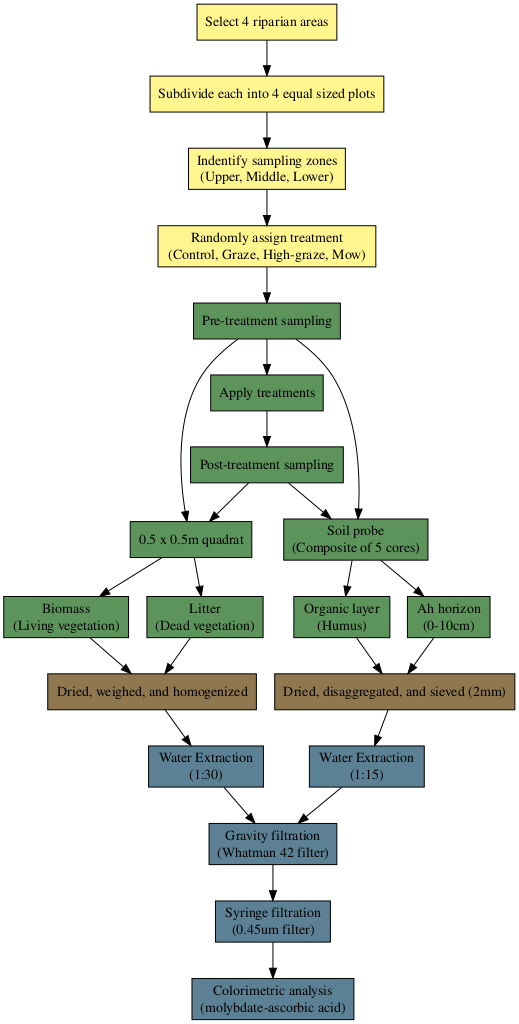
\includegraphics[keepaspectratio]{Workflow.png}}

}

\caption{\label{suppfig-workflow-plot}Workflow diagram showing the
experimental setup (yellow), field work (green), sample preparation
(brown), and laboratory analysis (blue).}

\end{suppfig}%

\begin{suppfig}

\centering{

\pandocbounded{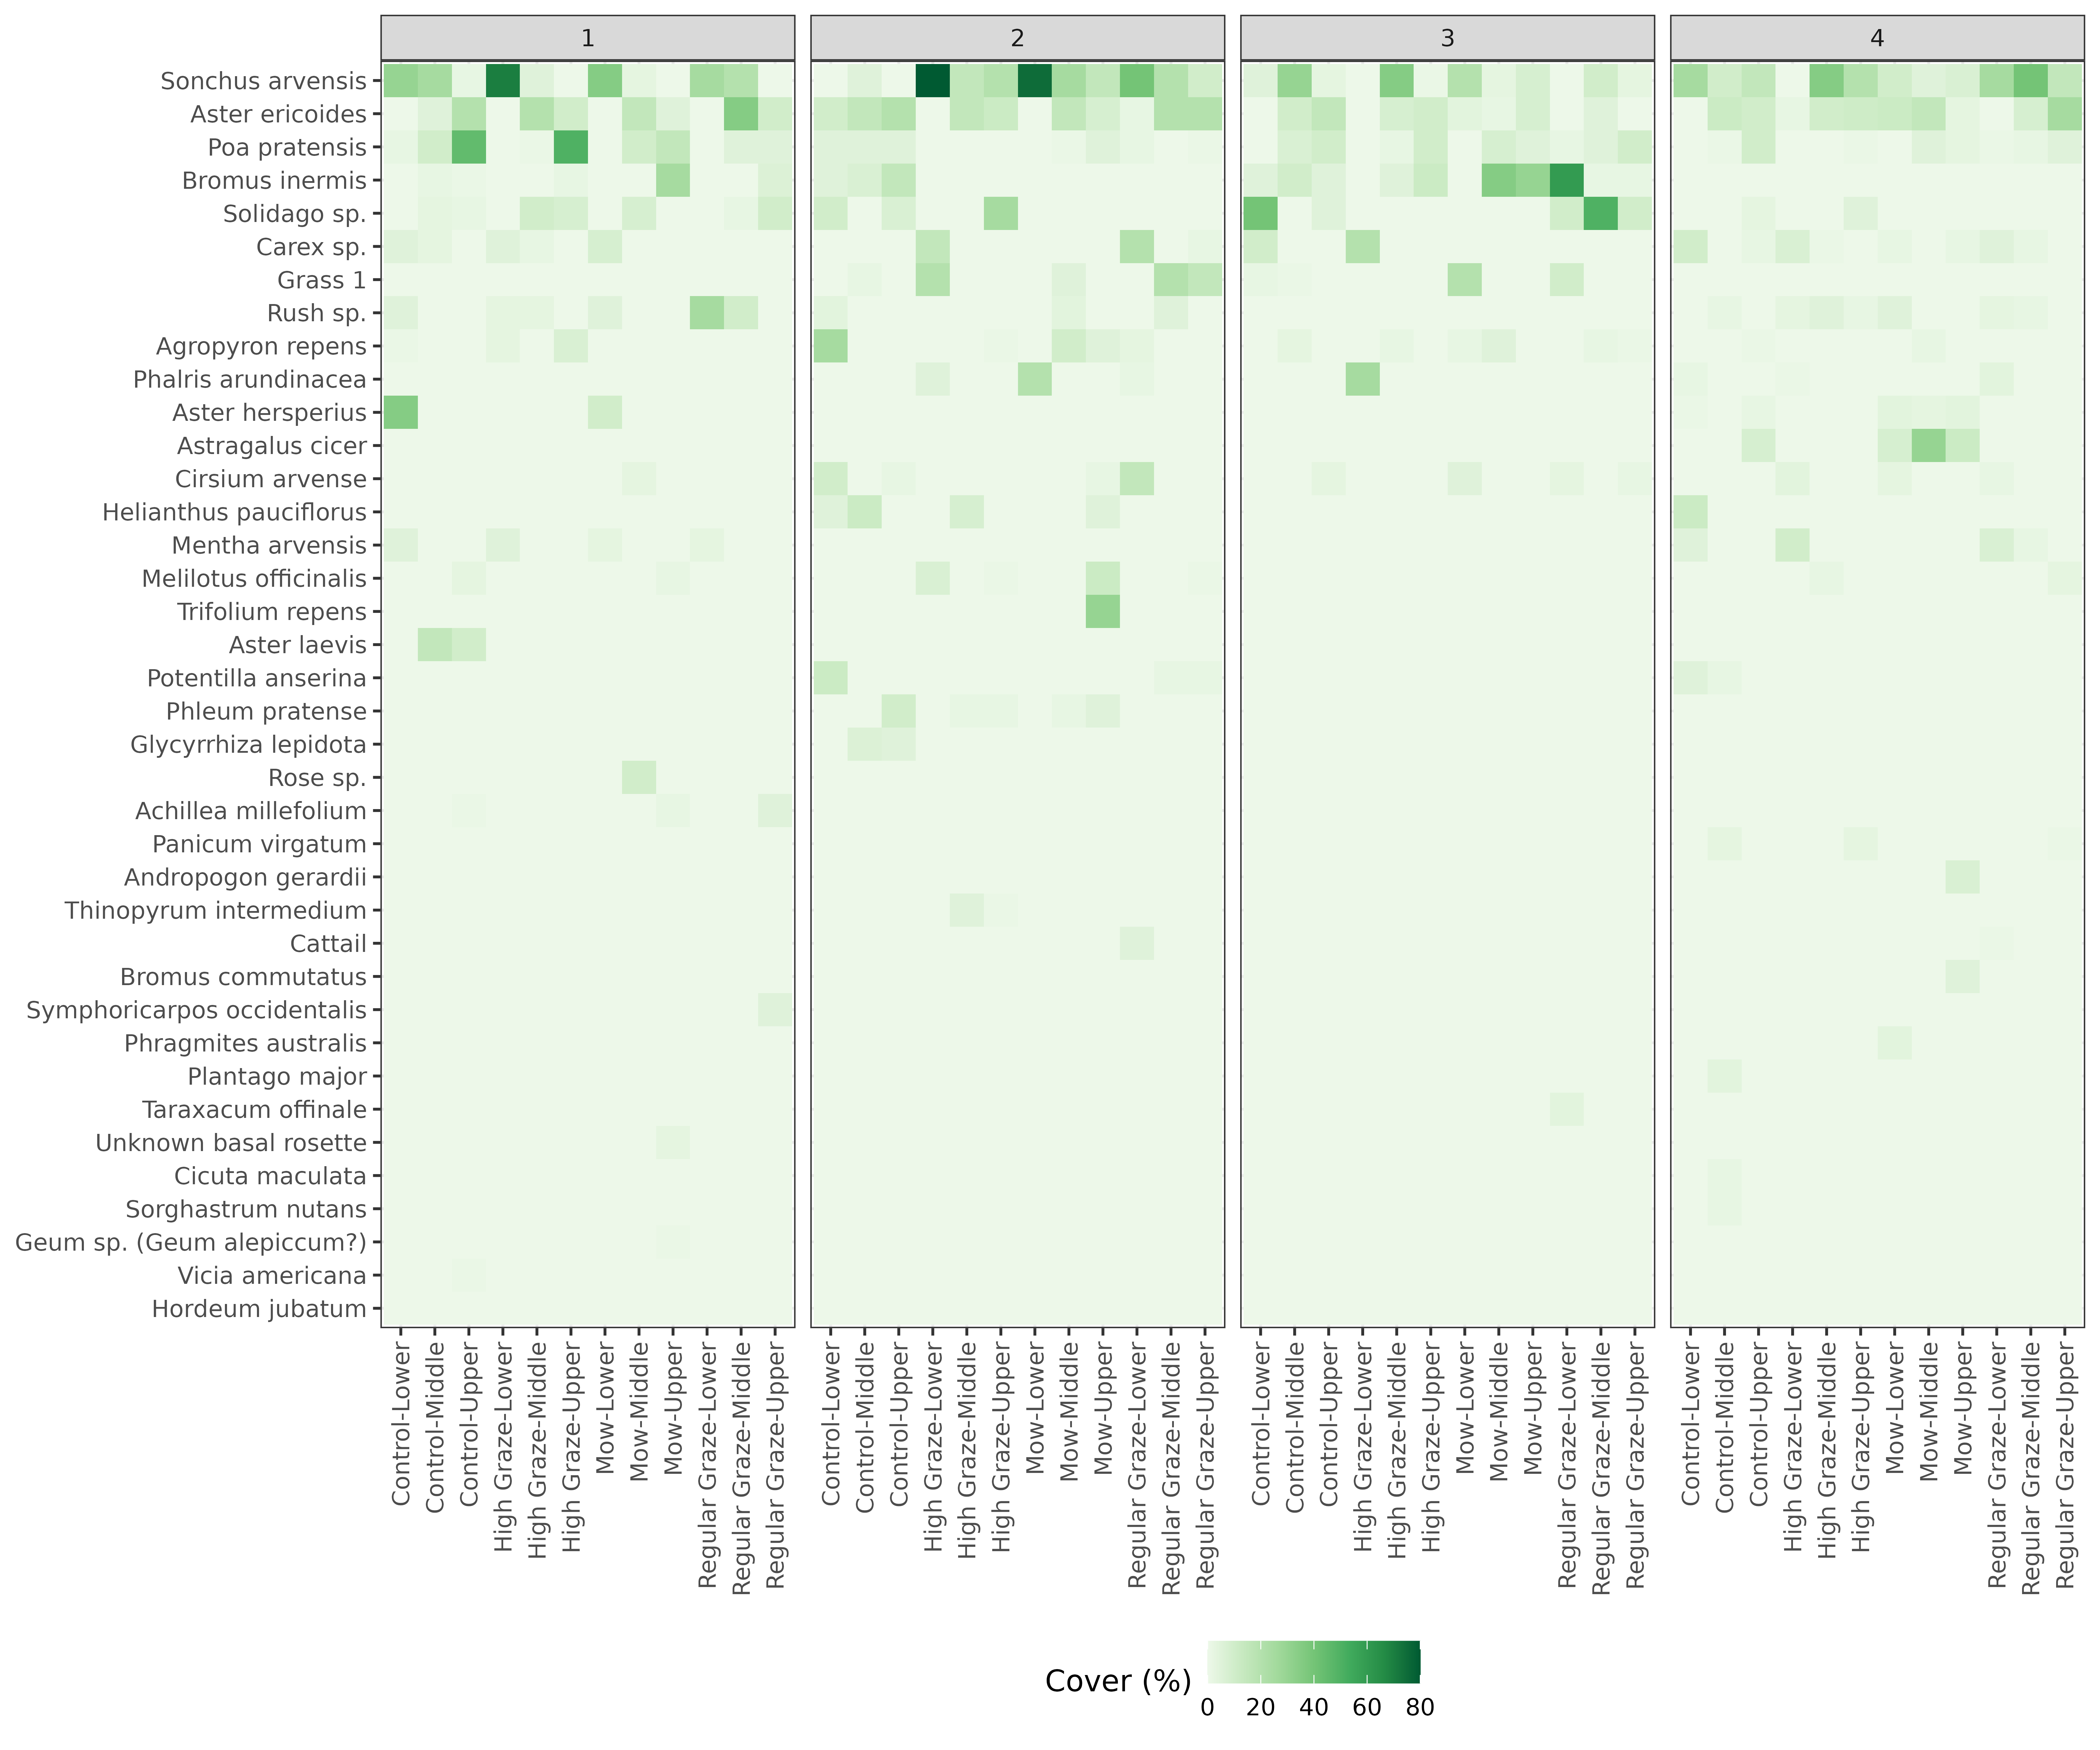
\includegraphics[keepaspectratio]{plant_composition.png}}

}

\caption{\label{suppfig-plant-plot}Initial year (2019) cover assessment
using the foliar cover method for each plot within the four riparian
locations}

\end{suppfig}%

\begin{suppfig}

\centering{

\pandocbounded{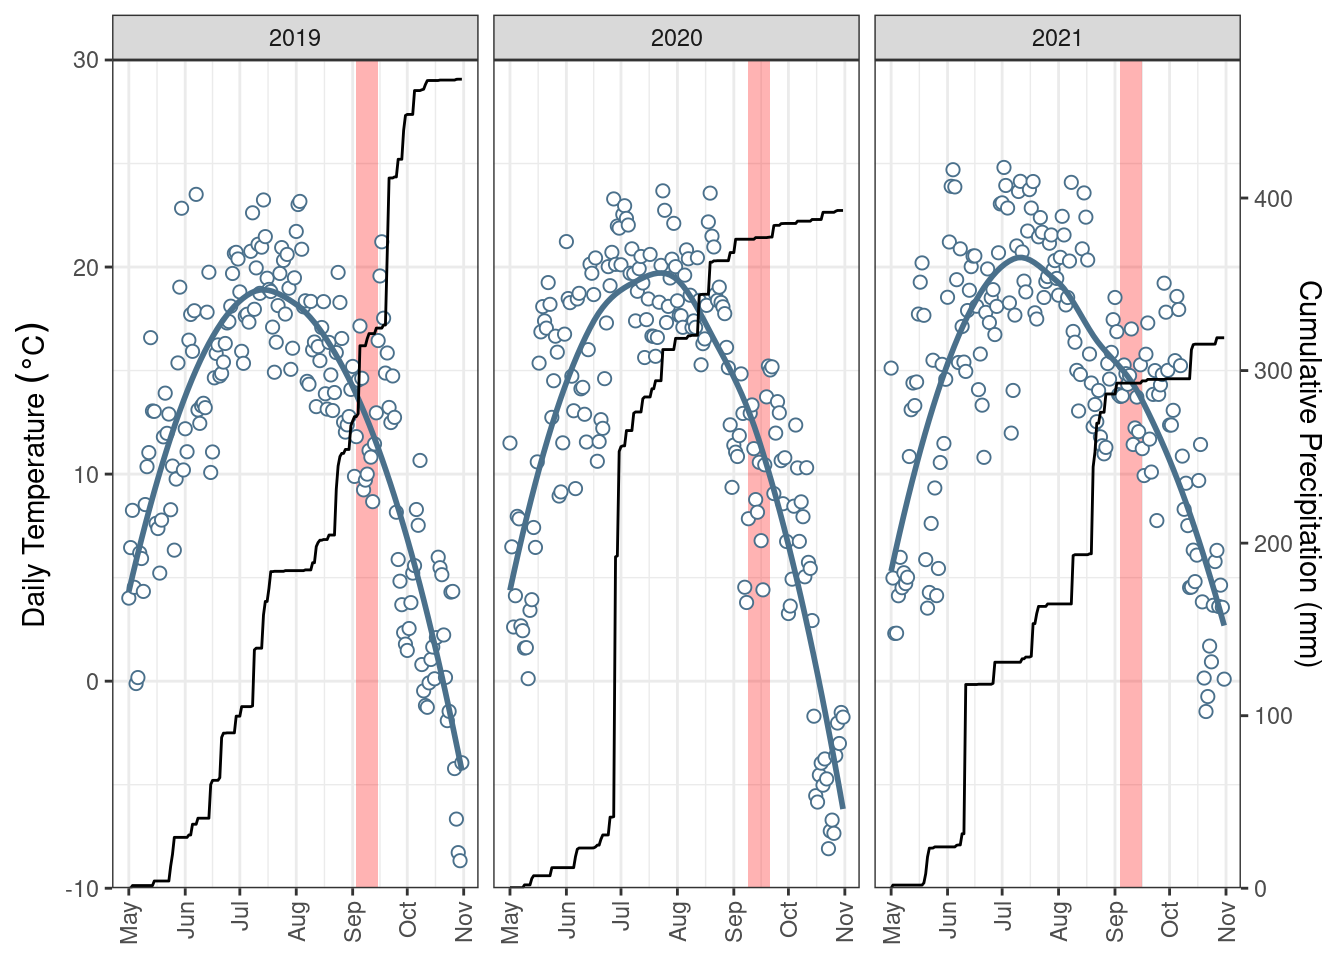
\includegraphics[keepaspectratio]{supp-weather-plot-1.png}}

}

\caption{\label{suppfig-weather-plot}Average daily air temperature and
cumulative rainfall over the growing season over the three year study.
Red bars indicate sampling dates}

\end{suppfig}%

\begin{suppfig}

\centering{

\pandocbounded{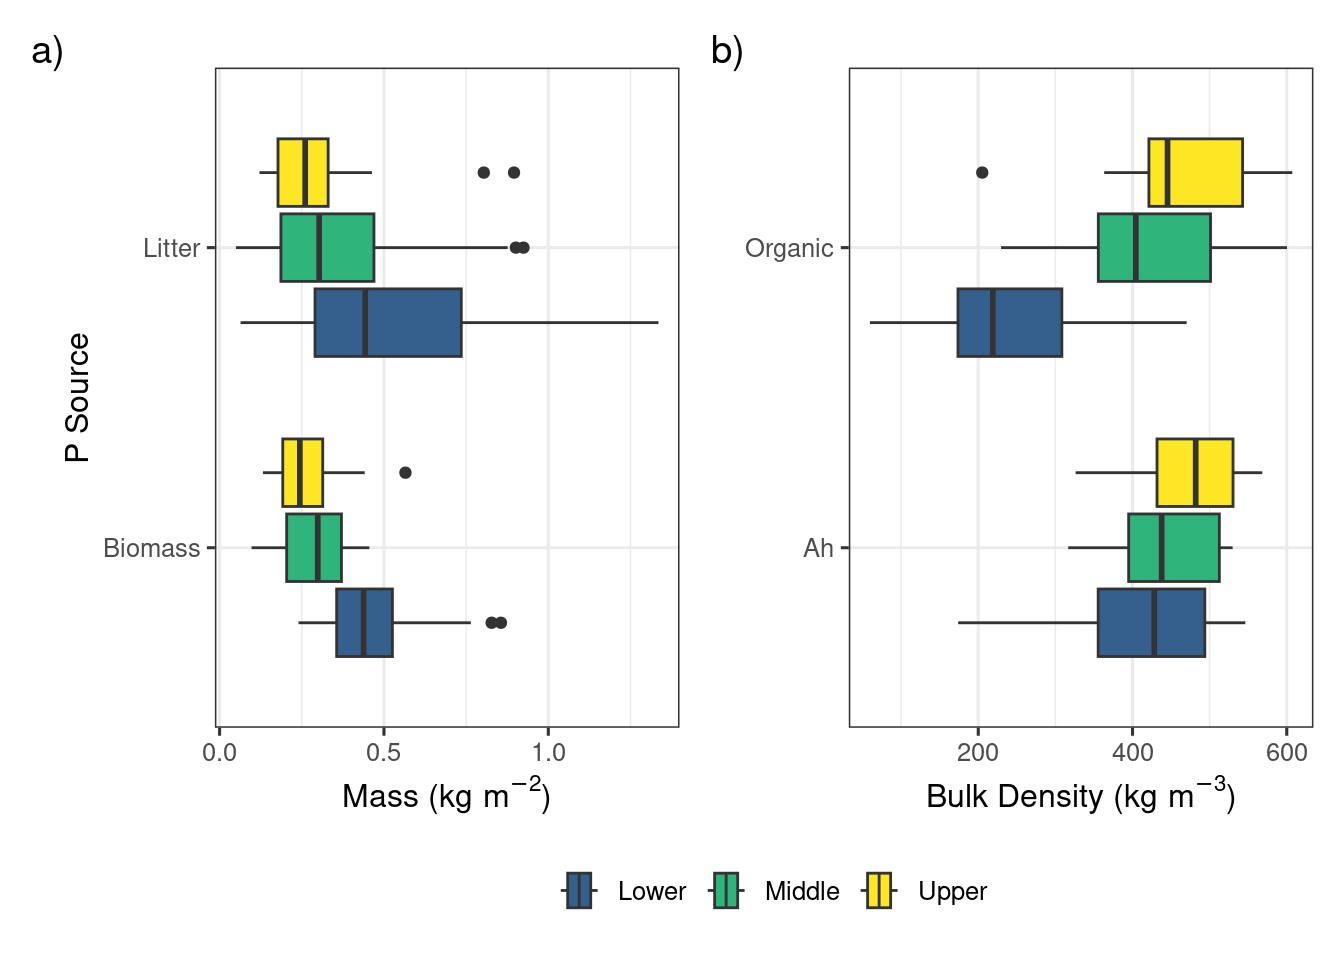
\includegraphics[keepaspectratio]{supp-weights-bd-1.png}}

}

\caption{\label{suppfig-bd-plot}a) Mass of biomass and litter before
grazing and mowing (2019-2021) and b) the bulk density of the organic
layer and 10 cm Ah horizon (2023)}

\end{suppfig}%

\begin{suppfig}

\centering{

\pandocbounded{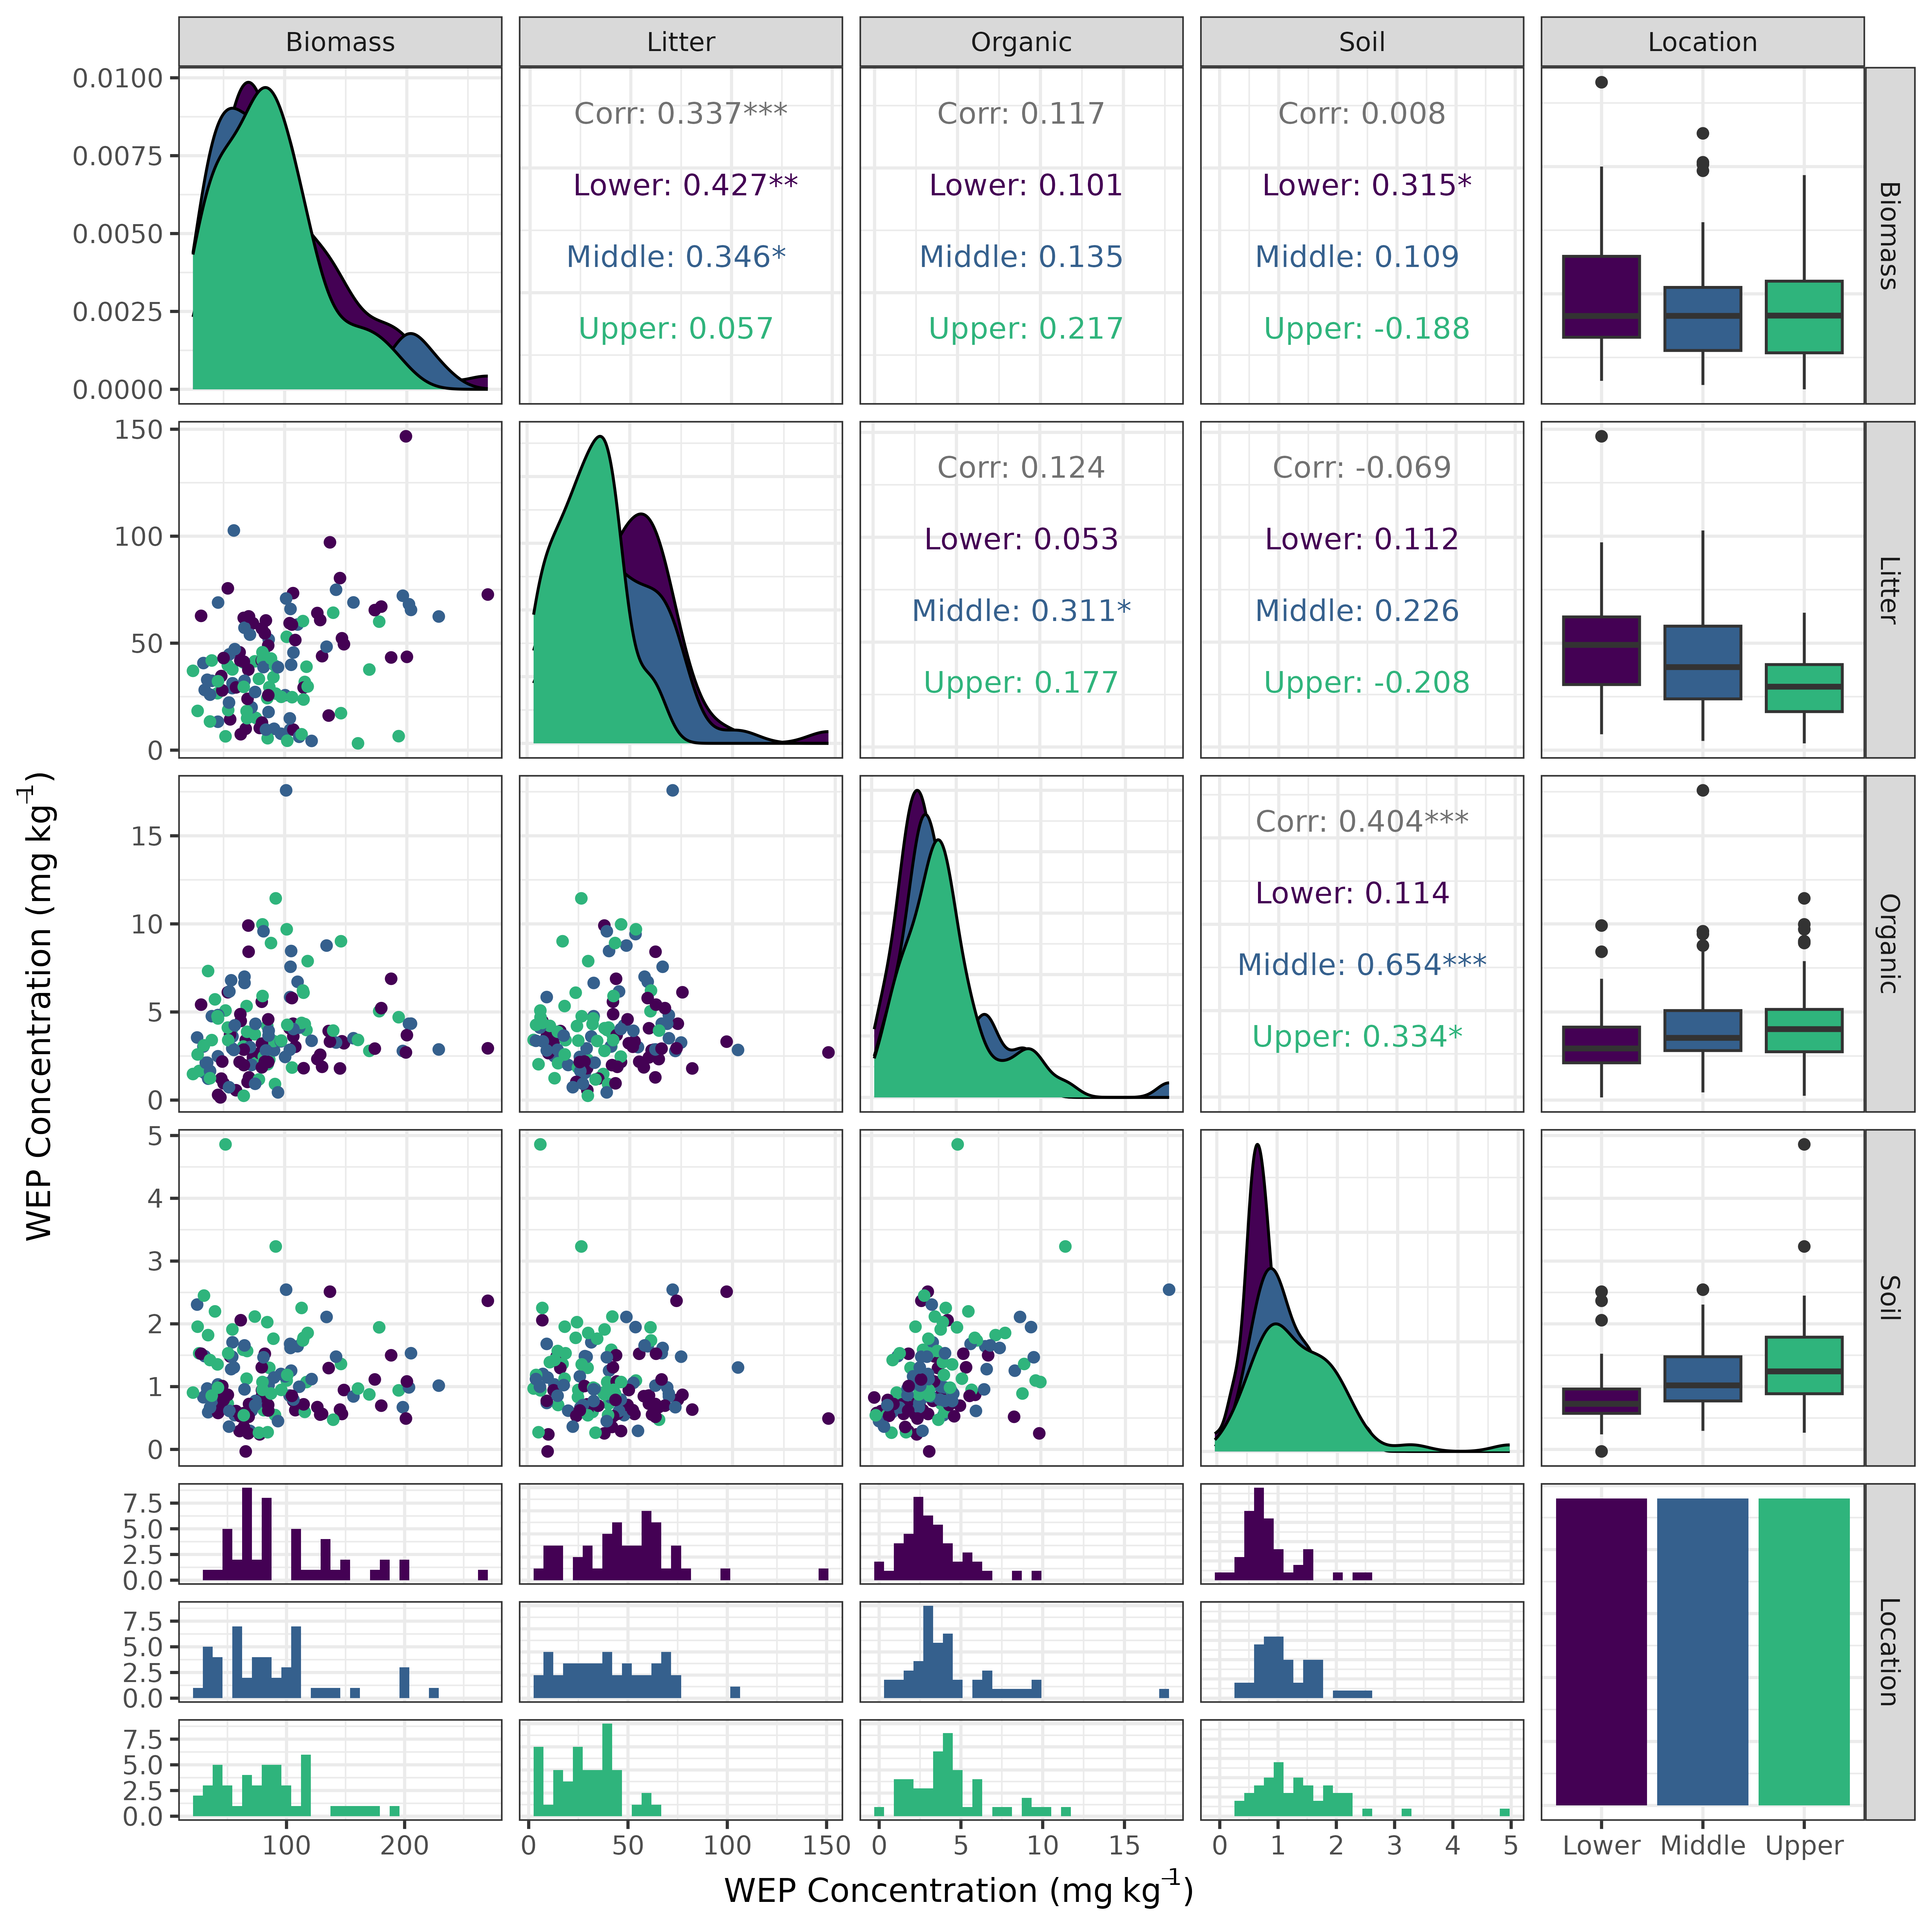
\includegraphics[keepaspectratio]{pair_plot.png}}

}

\caption{\label{suppfig-pairs-plot}Generalized pairs plot showing the
data and relationships between WEP concentration between the different
sources of Phosphorus at the lower (purple), middle (blue), and lower
(green) topographic positions. Data set only includes samples collected
before grazing and mowing treatments were applied. Corr indicates the
pearson correlation coefficient. *** p-value \textless{} 0.001, **
p-value \textless{} 0.01, ** p-value \textless{} 0.05.}

\end{suppfig}%

\begin{suppfig}

\centering{

\pandocbounded{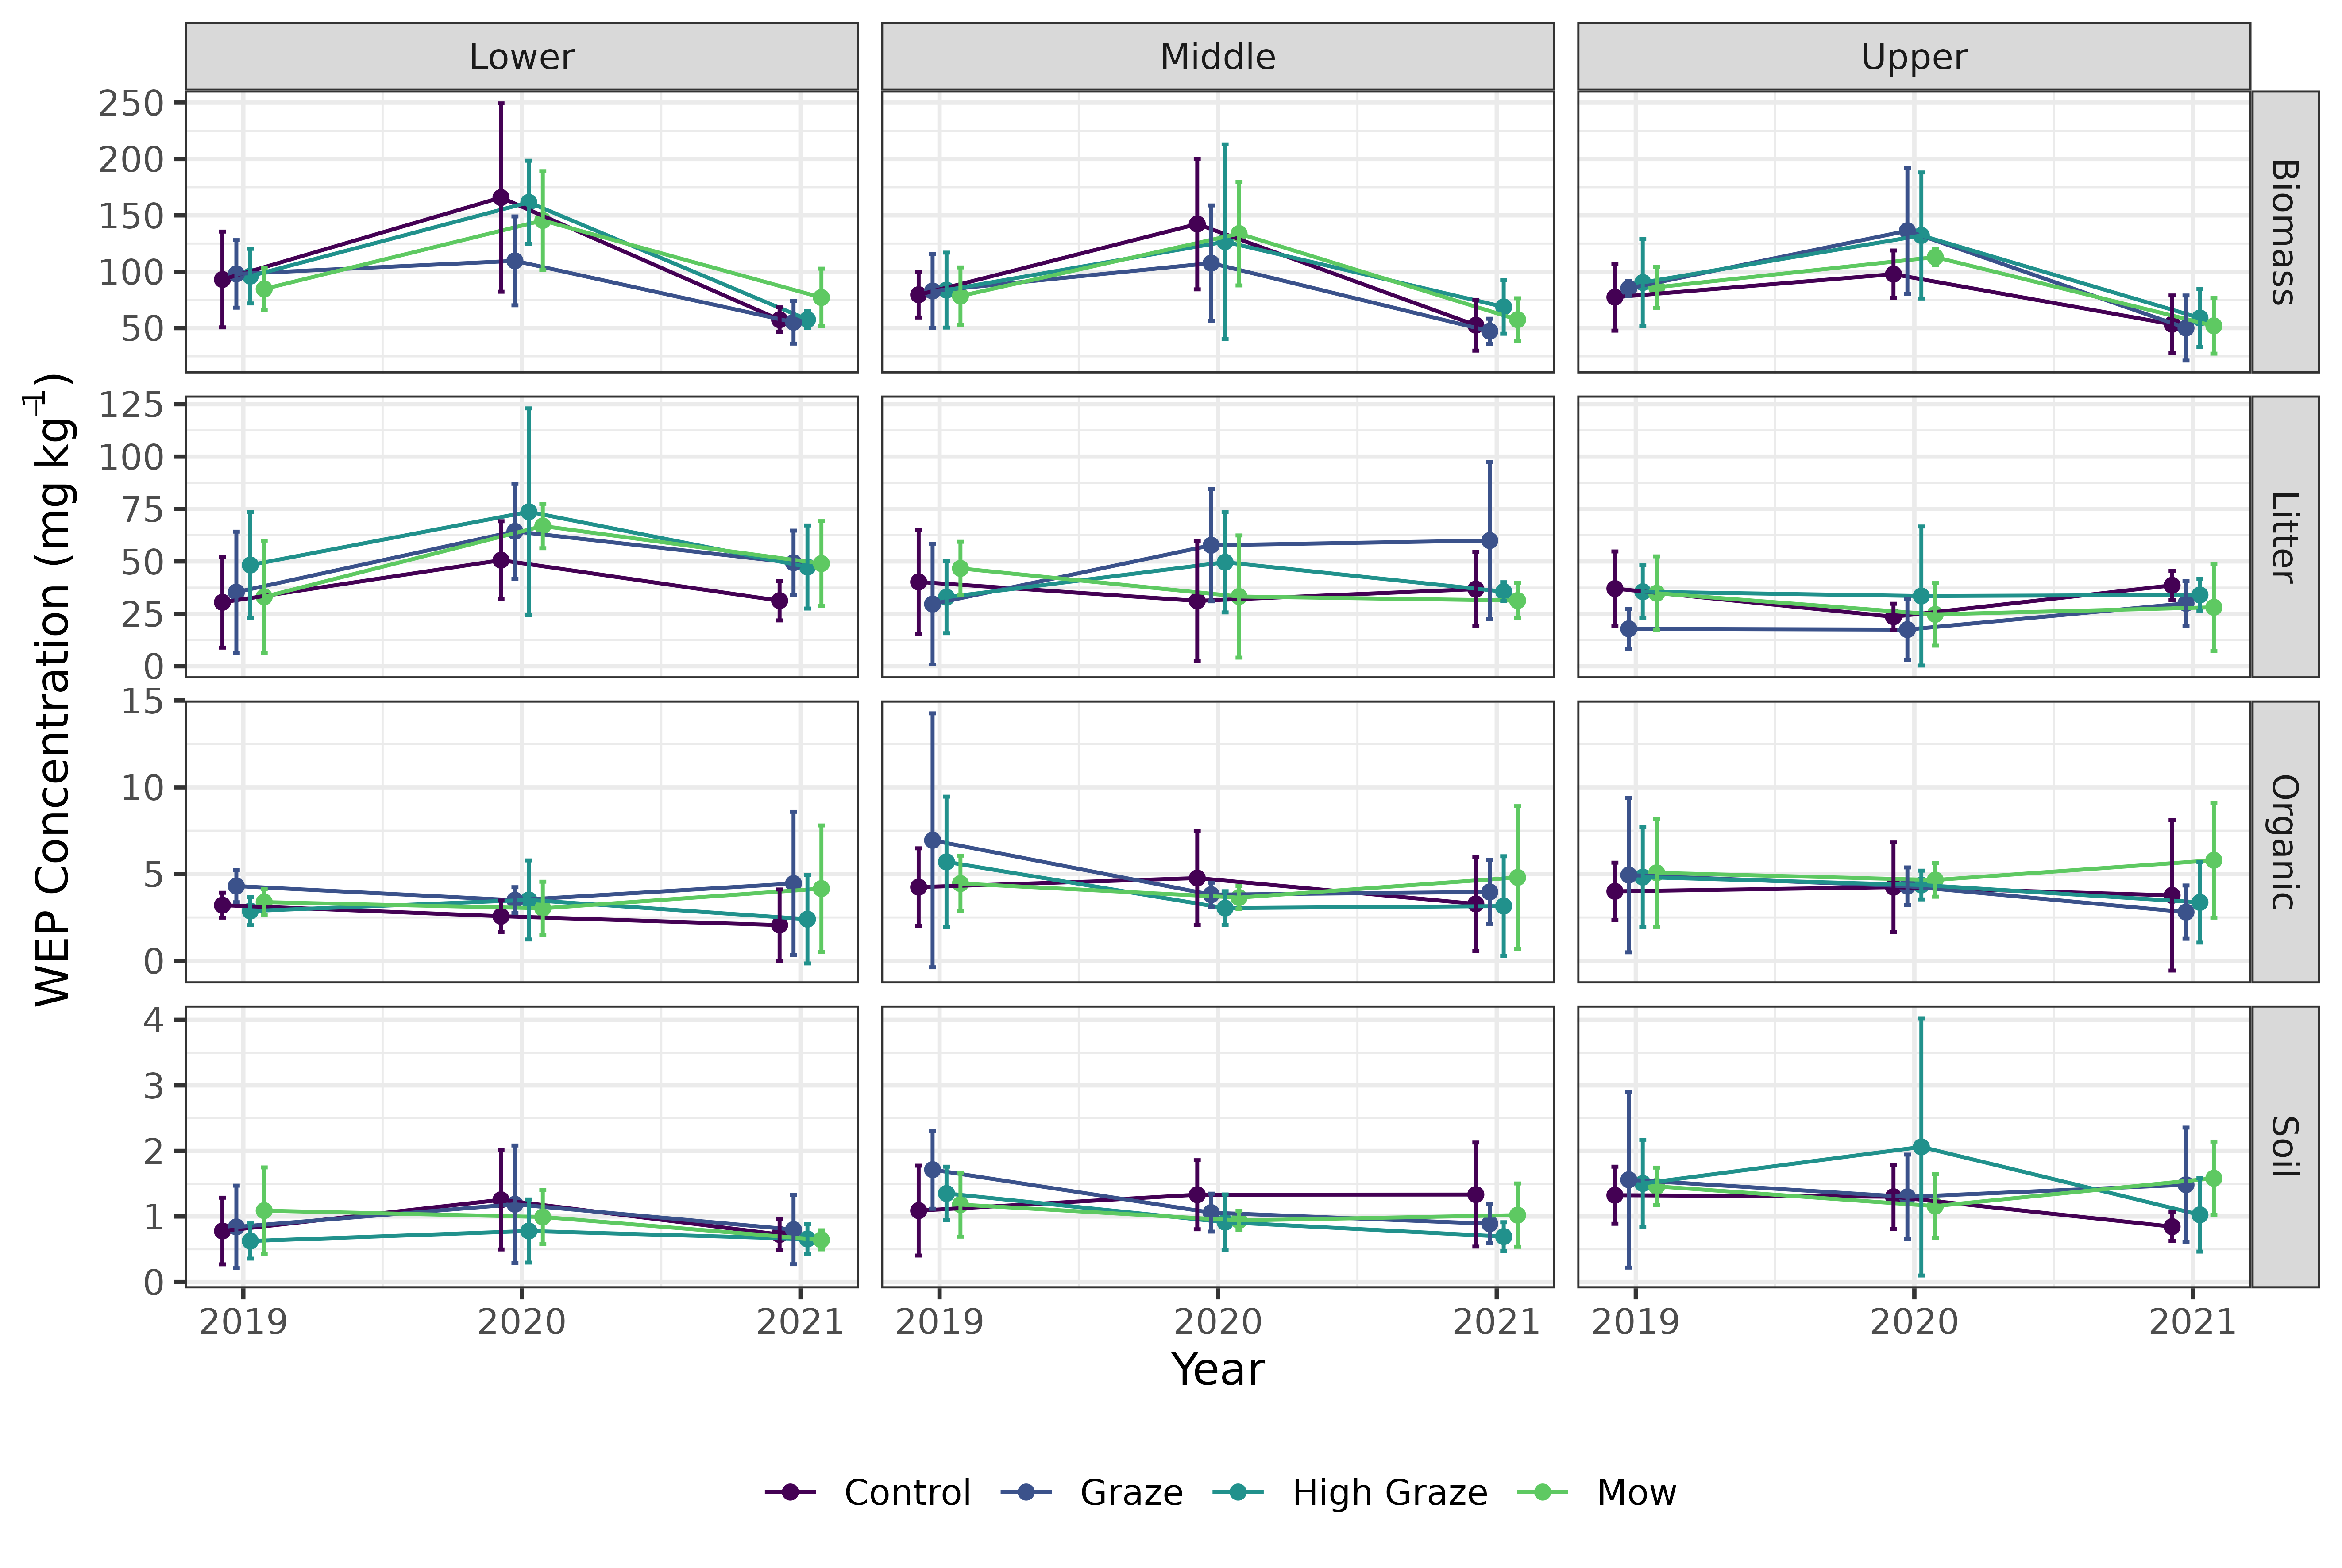
\includegraphics[keepaspectratio]{P_conc_year.png}}

}

\caption{\label{suppfig-years-plot}Mean and standard deviation WEP
concentration for each of the different sources of Phosphorus at each
topographic position over the three year period of observations. Data
set only includes samples collected before grazing and mowing treatments
were applied.}

\end{suppfig}%




\end{document}
